\documentclass[11pt]{scrartcl}

%\usepackage[utf8]{inputenc} % use UTF-8 as input encoding - not necessary with xelatex
%\renewcommand{\baselinestretch}{2} % Line height
\usepackage[T1]{fontenc} % make non-ASCII characters cut&pastable in PDF
\usepackage{lmodern} % easiest way to get outline fonts with T1 encoding
\usepackage[english=american]{csquotes} % automatic quotation style
\usepackage[american]{babel}
\usepackage{abstract}

\usepackage{amsmath,amssymb} % math
\usepackage{caption} % For caption*
\usepackage[hidelinks, colorlinks=true]{hyperref} % Make links from things

\usepackage{graphicx} % images
\DeclareGraphicsExtensions{.eps,.pdf,.png,.jpg,.gif}
\graphicspath{{./img/}}
\usepackage{tabularx} % tabulars
\usepackage{array,booktabs} % rules for frontpage
\usepackage{titling} % "vars" for titlepage
\usepackage{minted} % syntax highlighting
\usepackage{csquotes} % display quotes
\usepackage{cleveref}
\usepackage{framed}
\usepackage{array}
\newcolumntype{L}[1]{>{\raggedright\let\newline\\\arraybackslash\hspace{0pt}}m{#1}}
\newcolumntype{C}[1]{>{\centering\let\newline\\\arraybackslash\hspace{0pt}}m{#1}}
\newcolumntype{R}[1]{>{\raggedleft\let\newline\\\arraybackslash\hspace{0pt}}m{#1}}


% Setup the page geometry
\usepackage[a4paper,top=3cm,bottom=3cm,left=3cm,right=3cm]{geometry}
%\usepackage[a4paper,margin=5cm,top=3cm,bottom=3cm,left=2.7cm,right=2.7cm]{geometry}



\title{AURsec}
\newcommand{\titlesub}{Detecting and preventing targeted attacks in the Arch User Repository: A~blockchain-based~approach}
\author{Bennett Piater \& Lukas Krismer}
\newcommand{\leader}{Supervisor: Christian Sillaber}
\newcommand{\university}{University of Innsbruck}
\newcommand{\course}{Bachelor thesis}
\date{\today}

\begin{document}
  %%% Boilerplate
  \thispagestyle{empty}

  %frontpage
  \begin{titlepage}
    \noindent
    \begin{tabular}{@{}p{\textwidth}@{}}
        \toprule[2pt]
        \midrule
        \vspace{0.15cm}
        \begin{center}
            \Huge{\textbf{\thetitle}} \\
            \normalsize{\titlesub}
        \end{center}
        \vspace{0.15cm}\\
        \midrule
        \toprule[2pt]
    \end{tabular}
    \vspace{4 cm}
    \begin{center}
        \vspace{0.2cm}
        \LARGE{\theauthor} \\
        \vspace{0.1cm}
        %{\small \matrikel}
    \end{center}
    \vfill
    \begin{center}
        \course \\
        %\group \\
        \leader \\
        \vspace{1.2 cm}
        \university
    \end{center}
\end{titlepage}

  %  \vspace*{\fill}
\thispagestyle{empty}
  \begin{center} \textbf{\large{STATUTORY DECLARATION}} \end{center}
  I declare that I have authored this thesis independently, that I have not used other than the declared sources  /  resources,  and  that  I  have  explicitly  marked  all  material  which  has  been  quoted  either literally or by content from the used sources.

  \begin{center}
  \begin{table}[!htb]
  \begin{tabularx}{\textwidth}{lXX}
  Innsbruck 17.05.2017 & \_\_\_\_\_\_\_\_\_\_\_\_\_\_\_\_\_\_ & \_\_\_\_\_\_\_\_\_\_\_\_\_\_\_\_\_\_ \\
  Location,Date & Bennett Piater & Lukas Krismer \\

  \end{tabularx}
  \end{table}
  \end{center}
  \vspace*{\fill}
  \pagebreak 
f


  \pagenumbering{Roman}
  \begin{abstract}
    The Arch Linux User Repository is fundamentally insecure.
It was designed for simplicity and rapid iteration, leaving its users unprotected against many kinds of attacks.

This project increases its security by:
\begin{enumerate}
	\item Analyzing its security issues
	\item Creating a threat model
	\item Solving one of these issues, the \emph{lack of verified release checksums}, thereby protecting users against targeted attacks and compromised sources.
\end{enumerate}

For this purpose we compare the downloaded package sources with the hashes submitted by other users in a secure database where every user is allowed to upload each hash only once.
The database of choice was a blockchain capable of smart contracts because it is distributed and fulfills our security requirements.

  \end{abstract}

  \section*{Foreword}
  This thesis is written as part of the completion of the Bachelor of Computer Science (``Informatik'') by Bennett Piater and Lukas Krismer.

We chose this topic because we already used Arch Linux including the AUR and are generally interested in security. As users of the AUR we wanted to make it more secure, not only for us, but for all users.

\paragraph*{}

We want to thank Christian Sillaber for his supervision and
and our families and friends for their support.
We want to specially thank Justus Piater for his comments on how to improve the structure of the paper, Sara Bauer for her correction of our use of the English language, and Alad Wenter for his help during the integration with the AUR helper \texttt{aurutils}.

  \pagebreak


  \tableofcontents
  \listoffigures
  % \listoftables
  \pagebreak


  %%% Content starts here
  \pagenumbering{arabic}

  \section{Introduction}  %(1/2 page)
    \label{sec:intro}
The Arch Linux distribution constitutes a simple infrastructure which makes it easy to customize and participate in its development. As such, it provides packaging tools that facilitate the creation of custom packages and has attracted a very active community.
These facts necessitated the establishment of a place where active users could make their own packages available for others to use.

To address this issue, \texttt{ftp://ftp.archlinux.org/income} was created as a staging area; packages could be stored there until official maintainers would adopted them. However, waiting for the maintainers' participation implied a certain delay, so another solution was needed.
The next improvement constituted the \emph{Trusted User Repositories}, in which some privileged users, many more than the maintainers, were allowed to host their own repositories for anyone to use.

To completely remove the delay the \emph{Arch User Repository} (AUR) was created. The custom repositories were consolidated into one single repository, and the requirement to be a \emph{Trusted User} was dropped.
Thanks to the removal of all middlemen, everyone can now upload their packages to one central location. \cite{wiki:AUR}

The AUR is similar in design to PyPI (for Python), NPM (for Javascript) and rubygems.org, where all users can share their packages. All 4 platforms share a focus on simplicity, ease of use, and rapid iteration (creation of packages and roll-out of updates) at the expense of security.
The desire to allow anyone to use the system and to push out updates rapidly makes it hard to include proper vetting of contributors or auditing of software, thereby enlarging the possibility attacks.

\subsection*{Improving the Security of the AUR}
Most of the AUR's security issues are inherent to its design and thus cannot be solved without changing the AUR's concept in its entirety.
Nevertheless, some of them, which make users susceptible to targeted attacks through manipulated packages, can be remedied without modifying the AUR directly. That is the purpose of this paper.

Since targeted attacks only affect a small percentage of total users, they could be prevented by performing an additional integrity check which raises alarm if someone receives a different package than the majority of users.

This solution approach requires a tamper-proof, trust-less, preferably distributed database through which the most-seen hashes of a package can be tracked. Blockchains are a possible choice, as they fulfill all of these requirements.
Our tool \emph{aursec} hashes per-package information from the AUR and compares it to the most submitted hash of the corresponding package version stored in an Ethereum blockchain.
If the hashes differ, the user is warned of a possible attack.


% TODO: @important quick structure introduction?
% NOTE: I would ask christian
% Maybe ~one sentence about each section...

% Section 2 introduces blockchains, why we use one and why we chose Ethereum specifically.
% Section 3 is a threat assessment of the AUR including two concrete attack scenarios against which we want to defend.
% Section 4 describes our solution and implementation in detail.
% Section 5 lists some of the things we learned while working on our solution which may be of interest to readers.
% Section 6 discusses inherent qualities of our approach and compares it to other possible approaches.
% Section 7 evaluates our work by demonstrating how well we solved the problem that we set out to solve as well as discussing its usability and sensibility according to our experience and feedback from users.


  \section{Related Work}
    \label{sec:related}
\subsection{Arch}
Arch Linux \cite{wiki:arch} is a lightweight GNU/Linux distribution.
It was created by the Canadian Judd Vinet between 2001 and 2002 and further developed until today.
The renowned Arch Wiki was created in 2005. Since 2007 Aaron Griffin leads the development, which is completely done by part time volunteers in order to remain free from corporate influence.

Arch Linux follows the rolling-release model instead of periodical releases to provide the users the newest possible stable version of every program.
Upstream software is modified as little as possible and only as much as needed to integrate with the rest of the distribution.

Arch makes many features available earlier than other distributions, such as the systemd init system, software raids and new file systems.
Systemd \cite{wiki:systemd} replaced the \emph{System V init system} in 2013 \footnote{\url{https://bbs.archlinux.org/viewtopic.php?pid=1149530\#p1149530} accessed June 2, 2017}.
It provides a system- and service manager which starts the rest of the system and manages daemons and background services.
Systemd services are easy to handle and to configure.

Arch provides open-source packages as well as proprietary software to let the user decide if he wants functionality or if he wants to stay with the open-source ideology when they conflict.
Users can install them with the lightweight package manager \texttt{pacman}, which is one of the core tools of Arch.
Pacman uses a simple binary package format and an easy-to-use build system. It allows to manage the packages from the official repositories as well personal builds.

Arch is a lightweight distribution, which means that the user has to install and configure everything himself.
Arch does not want to be user-friendly, but rather user-centric.
This is achieved by providing the user with many possibilities to create his own personalized system and help him fix issues himself.
Arch encourages tinkering and caters to power users who want to understand and configure much of their system.
There are mailing-lists, an official Wiki, an official Forum, a bug tracker and several other places where users can get help.
Most members of the community are experienced Linux users who are willing to read documentations and solve problems on their own with the help of the community, as well as help others.

It is notoriously hard to estimate the popularity of Linux distributions, and so it is hard to tell how wide-spread Arch Linux is.
Arch users can voluntarily submit a list of their installed packages for statistical evaluation by installing and calling a script called \texttt{pkgstats}.
These stats show 13,353 different IP addresses from Arch users as of June 12, 2017~\cite{arch:stats}, which is fairly small.
However, no one knows how to control for administrators using many Arch machines behind one router, which seems to be common, and for the (probably many) users who do not submit these statistics.
According to the results of the yearly Reddit Linux Distribution Survey on \texttt{/r/linux} in 2015, 28.47\% of the participating users used Arch Linux~\cite{linuxsurvey}, with only Ubuntu appearing in the same order of magnitude.
Overall, it seems that Arch is a small, but very active distribution with comparatively vocal users. It's popularity has been steadily increasing for the past few years.

\subsubsection{AUR}
The Arch User Repository (AUR) is an unofficial, community-driven repository for Arch users.
It contains \texttt{PKGBUILD}s which are package descriptions containing all information needed to create packages from source using a tool called \texttt{makepkg}.
These packages can then be installed with \texttt{pacman}, Arches normal package manager.
Everyone can upload packages to the AUR as well as download them.
The uploaded packages are not verified or audited in any way in order to minimize the delay between the upload and the availability of a version.
Users can vote for packages; Packages with enough votes may get adopted by a maintainer and moved to the official Arch community repository.
If all maintainers of a package no longer want to maintain it, it can be orphaned. Any AUR user may adopt orphan packages.
\cite{wiki:AUR}

\subsection{Blockchain}\label{sec:ABCblockchain}
A blockchain is similar to a distributed database system which is not owned by a single user.
The first blockchain was implemented by Santoshi Nakamoto in 2008.
This blockchain is based on research of the early 1990s where the concept of cryptographically secured blocks was first described.
It is also the core of the bitcoin currency.
Since then several blockchain approaches where deployed.

As opposed to classic databases, blockchains maintain the entire transaction history.
Every user can look into this history and can track other users because the transactions are not anonymous.
Because of that, blockchains are the first digital approach of decentral database solving the double-spending problem.

Normally blockchain networks are peer-to-peer.
If a user wants to add a transaction to the blockchain, the transaction is encrypted, sent to all users, and verified.
If the majority of users validates the transaction, the data is added to the blockchain in the next block.
Underwood describes these transactions as ``... secure, trusted, auditable, and immutable''~\cite{Underwood}, which means that the transactions cannot be manipulated without a majority consent.

Users do not trust the result of a single node, but that of the majority.
As a result, blockchains are highly ``Byzantine''-fault tolerant.
This means that attackers need more than 50\% of the computation power to manipulate a blockchain (because then the attacker can produce more blocks than the rest).
If attackers gets more than 50\% of the computing power, they can manipulate the chain because the longest chain is always considered the canonical one.
Shorter tails become orphans and are rejected by the network.

Because blockchains are distributed and every user has a synchronized copy of the chain (which often requires several GB of disk space), they do not have a single point of failure or require backups.
The benefits of a blockchain compared to a conventional database are: (a) The blockchain can be directly shared because transactions contain their own proof as provided by a sophisticated cryptographic algorithm. (b) The blockchain is more robust (even than distributed databases).
Blockchains are often used to store transactions of concurrency (e.g. bitcoin), identity management or medical records.
\cite{Underwood,blockchain:eco}\newline\newline

To create new blocks \textbf{miners} are needed (proof of work).
A miner is the computer which has found a hash since the last block based on the transaction information and other data such as the hash of the last block.
This hash has to fulfill several requirements; The more there are, the more the mining difficulty increases.
It is hard to find a hash but it is easy to check if the hash fulfills all the requirements.
This is important because it makes it possible for every node to verify every block.

The mining difficulty describes the time effort required for mining of a block.
If the mining difficulty is high, the miner receives more \emph{coins} (Ethereum uses \emph{ether}) to reward the effort.
Coins are needed to perform transactions.
However, the effort and the payment have to be in sound relation to one another: that is, the miner's effort must not deceed or exceed the payment.
If the mining difficulty is too high in relation to the reward, it can lead to less blocks per hour which by implication leads to high transaction latencies because the transactions are not validated for considerable time.
If the opposite happens, there will be a low transaction per block ratio which makes the blockchain unnecessarily big; Users could also flood the chain with very many transactions, weakening the meaning of majority consent.\newline\newline

To provide functionality extending the transaction of coins, the blockchain has to accept \textbf{smart contracts}.
Smart contracts use computerized transaction protocols to execute the terms of a contract which are agreed upon by the users.
The term \emph{Smart Contract} might be misleading, as in reality it is a sequence of handling arrangements which map the contract clauses into code \cite{ecolex} --- they are effectively \emph{functions} of which the semantics may not be changed after all parties agreed on them.
Smart Contracts defining rules, penalties around an agreement and automatically check and impose them.

Without smart contracts, a blockchain can only handle the transaction of coins.
With smart contracts, a blockchain can be used as a database, containing objects which can be created, modified and deleted by \enquote{intelligent} transactions.
Additionally, object properties may be read without performing a transaction, allowing users to read information without paying currency.
The functions requiring coins are executed by every miner and are ACID transactions (atomic, consistent, isolated, durable).
Since the contract code is included in the chain, it is guaranteed to be immutable and therefore impossible to manipulate.
This guarantees that one is able to run secure code on the blockchain.

By avoiding middleman (e.g. lawyers), smart contracts are safer and often cheaper than their real-world counterpart.
They are safer because all parties communicate directly, and cheaper because the transaction fee is normally cheaper than the costs of a lawyer or notary.
Smart contracts can be used in different systems:
The Governments could use them for electronic voting systems, Companies already use them (e.g. Ethereum \footnote{\url{https://entethalliance.org/}) accessed on June 20, 2017}) in different ways and they are also used in healthcare systems (e.g. gem \footnote{\url{https://gem.co/} accessed on June 20, 2017}) which store the data in the blockchain and make it available for authorized users (e.g. doctors).
The healthcare-example also shows another advantage of smart contracts.
People cannot ``lose'' their data because its in the blockchain which is distributed.
Also Smart Contracts are more accurate than manually filled forms because they avoid manual errors.

Blockgeeks explains Smart Contracts with the following example:

\begin{displayquote}
	Suppose you rent an apartment from me. You can do this through the blockchain by paying in cryptocurrency. You get a receipt which is held in our virtual contract; I give you the digital entry key which comes to you by a specified date. If the key doesn’t come on time, the blockchain releases a refund. If I send the key before the rental date, the function holds it releasing both the fee and key to you and me respectively when the date arrives. The system works on the If-Then premise and is witnessed by hundreds of people, so you can expect a faultless delivery. If I give you the key, I’m sure to be paid. If you send a certain amount in bitcoins, you receive the key. The document is automatically canceled after the time, and the code cannot be interfered by either of us without the other knowing, since all participants are simultaneously alerted.~\cite{blockgeeks}
\end{displayquote}

Finally, one must mention that smart contracts are not perfect. Bugs in the code can lead to vulnerabilities which can be used to attack a blockchain.
The most popular example for this case is the ethereum-hard-split in 2016 \cite{heise-dao} where a bug in a smart contract was used to attack the Ethereum blockchain and steal 3,6 million ether-coins.
Furthermore, misunderstandings in traditional contracts can be fought over in court, but smart contracts cannot be modified or prevented from executing.
\cite{blockgeeks}


\subsection{Ethereum}
Ethereum is a blockchain-based, open-source, distributed computing platform developed by Vitalik Buterin, Gavin Wood and Jeffrey Wilcke.
It provides smart contract functionality. These smart contracts are usually written in the specially developed, Turing-complete language \emph{Solitidy}.
Solitidys syntax is similar to the syntax of JavaScript.
Every node runs an instance of the \emph{Ethereum Virtual Machine} (EVM), which can execute code of arbitrary complexity; The smart contracts are executed on the EVM.
Every EVM in the network executes the same instructions.

Ethereum rewards mining effort with it's currency, ether-coins.
As of June 3, 2017, the blockchains holds 92,2 Million Coins and is worth more than 20 billion US\$, which makes it the second most valuable blockchain after Bitcoin.
While every transaction in bitcoin costs exactly the same, transactions in ethereum have different fees based on the required storage, code complexity and bandwidth usage of smart contracts they interact with.
Beside it's main blockchain, Ethereum provides all the required infrastructure to create private blockchains.
\cite{ethereum, wiki:ethereum}

Bloomberg \cite{bloomberg:eth} describes Ethereum as \enquote{shared software that can be used by all but is tamperproof. You can safely do business with someone you don’t know, because terms are spelled out in a \enquote{smart contract} embedded in the blockchain. There could be blockchain versions of Uber and Airbnb that are peer-to-peer: No company would need to sit in the middle of the transaction to gather data about your spending habits or collect a fee.} %\cite{bloomberg:eth}


    \subsection{Other Approaches}
\emph{AUR helpers} have been developed to make the usage of the AUR easier.
They are designed to assist users with installing and updating packages from the AUR by automating some or all of the workflow (A detailed comparison can be found in the Arch Wiki~\cite{wiki:aur-helper}).
Some of them also give some degree of additional security compared to fully manual building.
In this section we want to look at \emph{yaourt}, \emph{bauerbill} and \emph{aurutils}.

Yaourt is the most popular AUR helper, but it is also one of the most insecure approaches~\cite{wiki:aur-helper}.
The user can use a command-line parameter to skip the only security layer, the manual \texttt{PKGBUILD}-check.
Users of Bauerbill and aurutils always have to check their \texttt{PKGBUILD}s.
Furthermore, aurutils makes the manual verification of \texttt{PKGBUILD}s easier by creating \emph{diffs} which show the changes between the last installed version and the current \texttt{PKGBUILD}.
Aurutils does not install the packages directly using pacman;
Instead, it adds or updates the package into a local repository.
These packages can be cryptographically signed by the user to ensure that they cannot be manipulated after they were created.
Pacman can then access this repository and install packages from it like from the official ones.
Bauerbill directly installs the packages after the \texttt{PKGBUILD}-check using pacman, but it displays if the maintainer of a package has changed since the last update.


  \section{Motivation: Security Issues of the AUR} %(1 1/2 pages)
    \label{sec:security_issues}
    \label{sec:motivation}
Ease of use appears to have been, if not the only, at least the primary design consideration of the Arch User Repository. This creates so many security issues that it is actually quite a task to address them all.

% PKGBUILDS
\subsection{Local Package Creation}
One of the most obvious problems is the installation procedure itself.
Arch packages are created locally from a bash file, the so-called \texttt{PKGBUILD} \cite{wiki:PKGBUILD}, containing metadata such as name and version, the URLs and checksums of upstream sources, and functions for the compilation and packaging steps.

The AUR contains these \texttt{PKGBUILD}s and possible patches to be applied to the upstream sources in a git repository per package.
A package file can be produced by cloning its repository and using a tool called \texttt{makepkg} \cite{wiki:PackageCreation}, which sources the script, downloads and verifies the sources, and calls the compilation and packaging functions.

This means that users can verify what they are compiling as opposed to blindly trusting binaries created by third parties; however, it also means that the maintainers of AUR packages have a means of executing arbitrary shell commands on users' machines.

This is aggravated by the fact that \texttt{PKGBUILD}s can include a \texttt{.install} file into the built package, which will be executed \emph{as root} when the package is actually installed.
The risk increases further if \emph{AUR helpers} are used, because some of them are unsafe in that they execute code before giving users the opportunity to inspect it, or disincentivize them from doing so.

\subsection{The Trust Issue}
Another problem is that users are not given any reason to trust the maintainers.
Unlike the official repositories, where maintainers are vetted, packages are (often manually) audited before being accepted, and everything must be signed with a trusted OpenPGP key, anyone can create an account and submit a new package to the AUR in a few minutes.
There is no admission procedure or audit system and no OpenPGP web of trust in order to minimize the time needed to publish a package or update.

\texttt{makepkg} can verify OpenPGP signatures for upstream sources, but the \texttt{PKGBUILD} itself could only be signed by using signed git commits, which is unfortunately not enforced or even officially recommended --- and not supported by any AUR helper anyway.

Except when using the AUR helper \texttt{bauerbill} \cite{bauerbill}, which provides a basic user-side trust management system (see Section~\ref{sec:security_comparison}), the only way to be maintain reasonable trust is to manually read every single file, which is cumbersome.
Since only security-conscious users are willing to put in so much effort before trusting a \texttt{PKGBUILD}, most users are left vulnerable.

\subsection{Adopting orphan packages}
The trust issue is aggravated by the fact that packages can silently and quickly be taken over by other maintainers due to the orphan/adoption system.

When maintainers want to stop maintaining a package, but the package is still useful and actively developed upstream, they have the option to \emph{orphan} it rather than deleting it.
Orphan packages can be \emph{adopted} by any AUR user, at any time, without delay.
This feature was designed to minimize update delay, which it does effectively; however, it also makes it easy for malicious agents to take over popular orphaned packages, manipulate them, and immediately orphan them afterwards.

\begin{center}
\begin{figure}
	\centering
	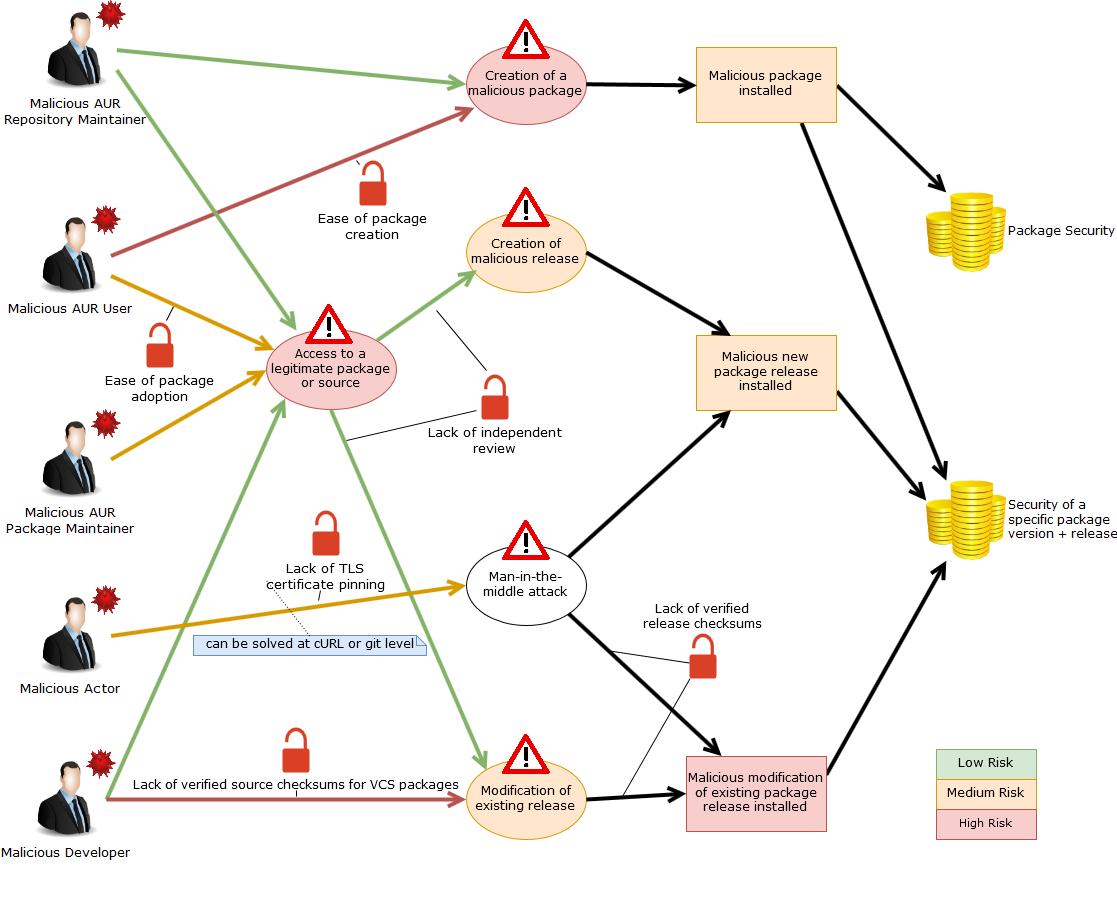
\includegraphics[width=\textwidth]{threat1n}
	\caption[Threat Assessment]{Threat Assessment of the Arch User Repository}
	\label{fig:threat}
\end{figure}
\end{center}

\subsection{Concrete Attack Scenarios}
\label{sec:attack_scenarios}
We used the CORAS \cite{Dahl:2007} threat modeling language to arrange the security issues in such a way that concrete attack scenarios are intuitive to comprehend and retrace. The resulting threat diagram can be seen in Figure~\ref{fig:threat}.

Many of the AUR's security issues, which emerged out of its design, are not easily solvable and are only included for completeness. However, Figure~\ref{fig:threat} shows that the vulnerabilities converge inwards and meet in only three points; This means that security issues further along the right of the diagram tend to be more promising candidates in the search for solvable problems.

This knowledge leads to two concrete attack scenarios that could be preempted without redesigning the AUR. These are outlined below.

% Threats:
\subsubsection{Tampered VCS Sources: Malicious Upstream}
\label{sec:vcs_attack}
In some cases, the user is not adequately protected against malicious (or compromised) upstreams:
The AUR supports so-called \emph{VCS packages} \cite{wiki:VCSPackages}, which download sources from a version control system, such as Git or Mercurial, instead of downloading a fixed archive. This relieves maintainers from updating their \texttt{PKGBUILD} for every new commit.
\texttt{makepkg} will even automatically calculate the up-to-date version number using for instance tags and commit numbers.

VCS packages were primarily designed to simplify the installation of up-to-date packages from source, and they do that well; however they also introduce a security issue:
Since the \texttt{PKGBUILD} does not need to be updated between versions, it cannot contain checksums for the new version either.
This used to be thought a small issue since most modern version-control systems use cryptographic hash functions for commit identification and integrity verification.
However, all popular ones use SHA-1, which has already been broken \cite{Stevens:2017}.
This means that attacks on VCS repositories using hash collision are possible.
In that light, users don't have a way to verify the authenticity of the source which they are downloading while building a VCS package, unless they can trust the upstream itself, meaning that no-one will notice if the upstream is compromised or makes malicious changes.
There is no way to counter this except to manually audit the upstream sources, which \emph{should} primarily be the maintainer's responsibility.

\subsubsection{Tampered Packages: Malicious Maintainer}
\label{sec:maint_attack}
Users are also not adequately protected against malicious maintainers:

Because it is easy to gain access to a package, e.g. by adopting an orphan or simply by creating it, and nothing is verified or audited before publication, it is easy for a malicious agent to modify a package.
Additionally, since the \texttt{PKGBUILD} is not signed or hashed, users will not notice if the build instructions for a specific package version were modified. This allows targeted attacks:

If the time at which targets will update their machine is known and one has access to an AUR package which they expected to update, malicious code can be introduced into the corresponding \texttt{PKGBUILD} or \texttt{.install} files within that update window.
This could be as simple as changing the checksum if one also has access to the upstream source code (even a very careful user has no chance of noticing this attack), or executing innocuous code in the install file or \texttt{PKGBUILD} itself.

The malicious change could be reverted immediately afterwards. If the time frame is short, no other AUR user (and thus, \emph{no-one}) would ever notice.
One can only defend against this with a good local trust model, such as that possible with \texttt{bauerbill}, or manual cryptographic verification of the git commit to the AUR, if the attack was conducted by adopting an orphan package --- assuming that the maintainer signs his commits, which is only rarely the case.
 % BENNETT

  \section{AURsec}
    % TODO: maybe main tool - aursec; initialization - aursec-init; API - aursec-chain
    \label{sec:AURsec}
\begin{figure}
	\centering
	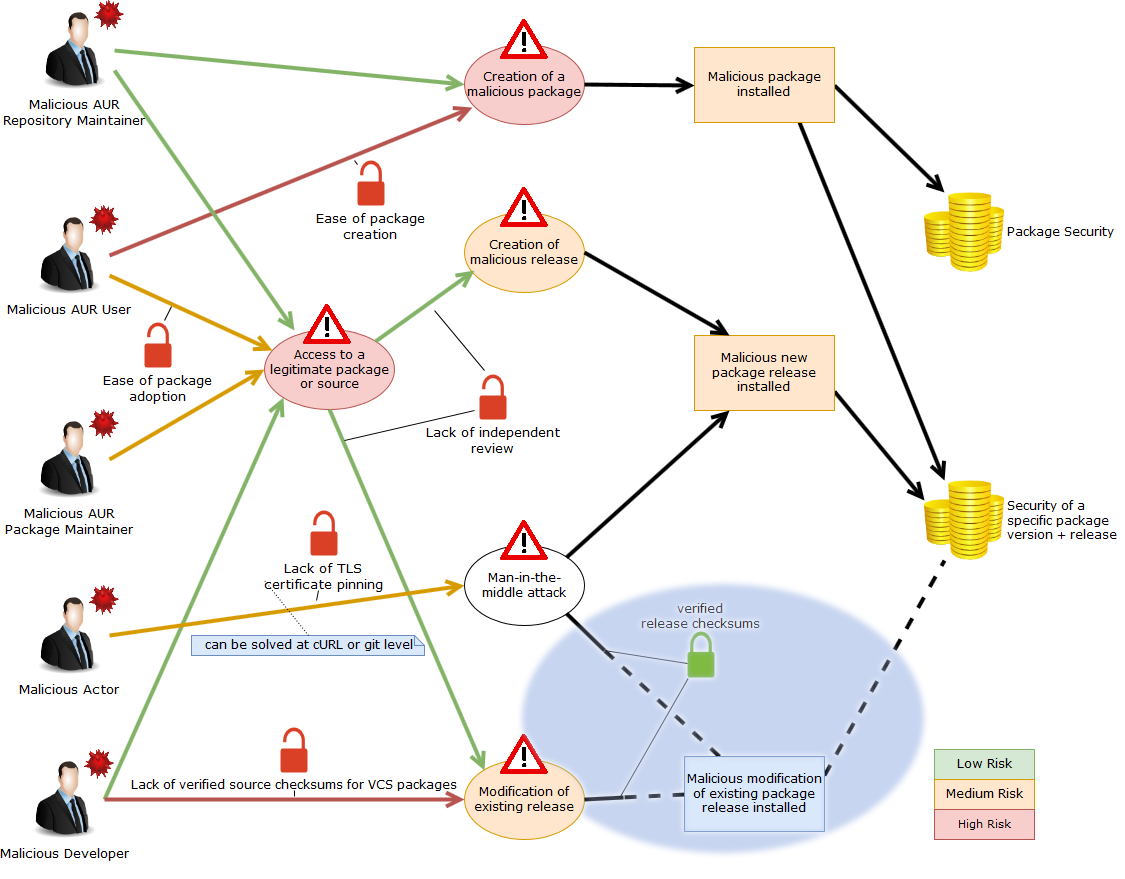
\includegraphics[width=\textwidth]{threat2n}
	\caption[Threat Prevention Strategy]{Strategy for Improving the Security of the AUR}
	\label{fig:threat2}
\end{figure}

Defence against the two attack scenarios mentioned in Section \ref{sec:attack_scenarios} requires the availability of cryptographically secure release hashes for every version of every package (Figure \ref{fig:threat2}).
If those were available, an attack would result in a hash mismatch and therefore the user could be warned.
However, the focus of the AURs design on simplicity, automation and fast package updates prevents any secure implementation on the server side as it would require the introduction of a central point of trust. That trust could only be maintained through the introduction of manual auditing, which is the opposite of what the AUR was designed for.

The solution must therefore be to implement a (preferably distributed) database on the user side, which means that there is no single authoritative source.
Since the aim is to defend against \emph{targeted} attacks, the assumption being that only comparatively few users will encounter a malicious version, this can be circumnavigated by checking the hash against a \emph{consensus} formed by many users.

% TODO: @important @lukas @bennett This paragraph is probably still unclear... need to think about that!
To make the database as safe as possible, a blockchain is used. The chain contains a smart contract providing securely callable functions. With one of these functions it is possible to commit a hash for a specific package and version.
This hash will be saved in the blockchain only if this user has not committed the same hash before, thereby making it harder to take over the blockchain and get a malicious hash to be the consensus.
The consensus is updated after every hash commit. Another function is used to get the current consensus hash and its valid commit count for a specific package and version.

This is the first project to use a blockchain as a means to provide distributed verification of (software) downloads.

% Workflow
\subsection{Workflow}
\label{sec:workflow}
The following workflow is visualized in Figure \ref{fig:main_workflow}.
\begin{figure}[!htb]
	\centering
		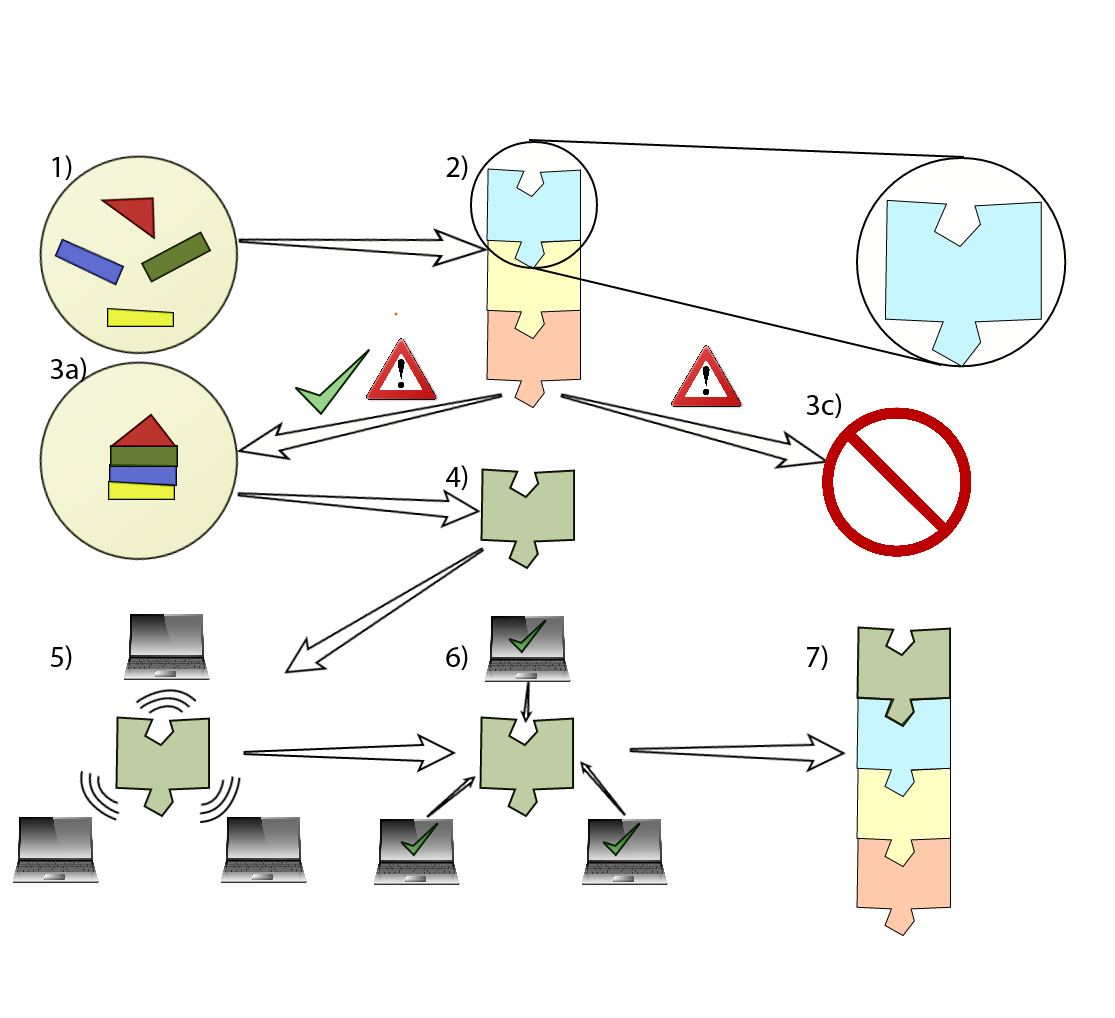
\includegraphics[width=0.6\paperwidth]{Workflow2}
	\caption{Main (Blockchain) Workflow}
	\label{fig:main_workflow}
\end{figure}

\begin{figure}[!htb]
	\centering
		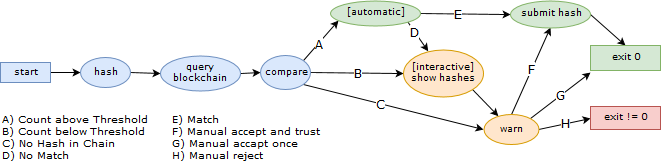
\includegraphics[width=\textwidth]{decision2}
	\caption{Aursec State Machine}
	\label{fig:state_machine}
\end{figure}


First of all a \texttt{PKGBUILD} is downloaded and partially executed in a sandbox in order to get the package version and download VCS sources (1).
Then, it is hashed along with any VCS sources and \texttt{.install} files.
The resulting local hash is compared with the current consensus (most often committed) hash of this package-version on the blockchain (2).

Depending on the comparison of the hashes (3), one of three things will happen [Figure~\ref{fig:state_machine}]:
The package may be created, installed and the hash will be added to the blockchain \emph{(Followed by step 4)} if the hashes match and the number of commits is above the trust threshold or the user decides to trust the locally generated hash anyway (A, F).

The package may be created and installed but the hash will not be added to the blockchain if the hashes do not match and/or the number is below the threshold, but the user wants to create and install the package without committing the hash. In this case the program exits with a zero status (B \rightarrow~G).

The package may not be created and installed because the hashes do not match and/or the number is below the threshold and the user doesn't want to create the package. In this case the program exits with a non-zero status (H).

If the locally generated hash is trusted, the local hash is committed to the blockchain (4). This is a transaction [see \texttt{aursec-chain commit-hash)}].
All nodes in the blockchain get the transaction over the network (5) and the transaction will be verified (together with all other transactions since the last block) and included the next mined block (6).
This mined block is then added to the blockchain (7).
As the transaction is included in a mined block, the consensus is atomically updated to reflect the new hash submission.
 %LUKAS
    \subsection{Blockchain implementation}\label{sec:aur-block}
In our approach we used Ethereum as blockchain and Solidity as the programming language for the smart contract.
We have chosen Ethereum because our blockchain has to fulfill several requirements:

Since we target Arch Linux, it must be easy to install on this platform.
This is covered by the \emph{geth} package which is available in the official community repository and can be directly installed using pacman.
The blockchain also needs to provide an API which allows external scripts to work with it.

Ethereum provides two APIs:
An IPC (interprocess communication) API, which allows connecting an interactive \emph{geth} console to a running blockchain, but is not convenient for external scripts,
and an HTTP RPC (remote procedure call) API which allows to send HTTP requests containing JSON bodies.
These requests can be sent with external scripts and programs since nearly every programming and scripting language (including bash) has HTTP support.
In our approach the shell script \texttt{aursec-chain}~(Section~\ref{sec:aursec-chain}) and the Python script \texttt{aursec-tui}~(Section~\ref{sec:tui}) use this API to interact with the blockchain.

The blockchain also needs to support smart contracts in order to allow us to use the blockchain functionally.
Ethereum not only supports smart contracts, they are it's main feature.
The specially developed high-level language \emph{Solidity} allows to write smart contracts in little time.

Our smart contract (Appendix~\ref{sec:contract}) provides two public functions which allow users to submit hashes (line 56) and to request the current consensus hash of a versioned package (line 43).
The contract allows each user to commit a hash only once: further commits of the same hash by the same user will not be considered in order to prevent manipulation of the consensus. This is implemented by keeping track of who submitted a hash (lines 58-60).

Finally, the blockchain needs to to provide an easy way to create private networks separate from the main one.
It would be safer to use the main blockchain because larger chains are harder to manipulate, and miners would get currency worth real money (in addition to secure software downloads) for their work, but we decided against that because the main blockchain takes up a lot of disk space and has much higher mining costs than makes sense for our application.
Ethereum provides possibilities to create private networks easily; It is only required to choose a network ID and to host the bootnode that is required to build the peer to peer network.
Our bootnode is active 24/7 on a DigitalOcean droplet provided by our supervisor.
Appendix \ref{sec:init-boot} explains how a new bootnode is added to the aursec-network.
 % LUKAS
    \subsection{Initialization - aursec-init}\label{sec:aursec-init}
Aursec-init is a shell script which allows the user to create all requirements for using our project.
It can also be used to rebuild the local copy of the blockchain, effectively re-installing from scratch.

First, it creates all needed folders and markers.
These markers track when hash commits and mining take place and are used by the systemd-service \textit{aursec-blockchain-mine} to adjust the mining effort based on recent hash commits.
Then, it creates the blockchain from our \emph{genesis block}, which is the first block in the blockchain.
After that, the synchronization of the blockchain begins.
In the meantime, the generation of the first two \emph{Directed Acyclic Graphs} (DAG) is stated.
Every DAG is a \~1GB dataset which is needed for mining new blocks \cite{wiki:DAG}.
Finally, the script mines a few blocks to gain enough currency to enable committing of hashes right after the initialization.
 % LUKAS
    \documentclass[11pt]{scrartcl}

%\usepackage[utf8]{inputenc} % use UTF-8 as input encoding - not necessary with xelatex
%\renewcommand{\baselinestretch}{2} % Line height
\usepackage[T1]{fontenc} % make non-ASCII characters cut&pastable in PDF
\usepackage{lmodern} % easiest way to get outline fonts with T1 encoding
\usepackage[english=american]{csquotes} % automatic quotation style
\usepackage[american]{babel}
\usepackage{abstract}

\usepackage{amsmath,amssymb} % math
\usepackage{caption} % For caption*
\usepackage[hidelinks, colorlinks=true]{hyperref} % Make links from things

\usepackage{graphicx} % images
\DeclareGraphicsExtensions{.eps,.pdf,.png,.jpg,.gif}
\graphicspath{{./img/}}
\usepackage{tabularx} % tabulars
\usepackage{array,booktabs} % rules for frontpage
\usepackage{titling} % "vars" for titlepage
\usepackage{minted} % syntax highlighting
\usepackage{csquotes} % display quotes
\usepackage{cleveref}
\usepackage{framed}
\usepackage{array}
\newcolumntype{L}[1]{>{\raggedright\let\newline\\\arraybackslash\hspace{0pt}}m{#1}}
\newcolumntype{C}[1]{>{\centering\let\newline\\\arraybackslash\hspace{0pt}}m{#1}}
\newcolumntype{R}[1]{>{\raggedleft\let\newline\\\arraybackslash\hspace{0pt}}m{#1}}


% Setup the page geometry
\usepackage[a4paper,top=3cm,bottom=3cm,left=3cm,right=3cm]{geometry}
%\usepackage[a4paper,margin=5cm,top=3cm,bottom=3cm,left=2.7cm,right=2.7cm]{geometry}



\title{AURsec}
\newcommand{\titlesub}{Detecting and preventing targeted attacks in the Arch User Repository: A~blockchain-based~approach}
\author{Bennett Piater \& Lukas Krismer}
\newcommand{\leader}{Supervisor: Christian Sillaber}
\newcommand{\university}{University of Innsbruck}
\newcommand{\course}{Bachelor thesis}
\date{\today}

\begin{document}
  %%% Boilerplate
  \thispagestyle{empty}

  %frontpage
  \begin{titlepage}
    \noindent
    \begin{tabular}{@{}p{\textwidth}@{}}
        \toprule[2pt]
        \midrule
        \vspace{0.15cm}
        \begin{center}
            \Huge{\textbf{\thetitle}} \\
            \normalsize{\titlesub}
        \end{center}
        \vspace{0.15cm}\\
        \midrule
        \toprule[2pt]
    \end{tabular}
    \vspace{4 cm}
    \begin{center}
        \vspace{0.2cm}
        \LARGE{\theauthor} \\
        \vspace{0.1cm}
        %{\small \matrikel}
    \end{center}
    \vfill
    \begin{center}
        \course \\
        %\group \\
        \leader \\
        \vspace{1.2 cm}
        \university
    \end{center}
\end{titlepage}

  %  \vspace*{\fill}
\thispagestyle{empty}
  \begin{center} \textbf{\large{STATUTORY DECLARATION}} \end{center}
  I declare that I have authored this thesis independently, that I have not used other than the declared sources  /  resources,  and  that  I  have  explicitly  marked  all  material  which  has  been  quoted  either literally or by content from the used sources.

  \begin{center}
  \begin{table}[!htb]
  \begin{tabularx}{\textwidth}{lXX}
  Innsbruck 17.05.2017 & \_\_\_\_\_\_\_\_\_\_\_\_\_\_\_\_\_\_ & \_\_\_\_\_\_\_\_\_\_\_\_\_\_\_\_\_\_ \\
  Location,Date & Bennett Piater & Lukas Krismer \\

  \end{tabularx}
  \end{table}
  \end{center}
  \vspace*{\fill}
  \pagebreak 
f


  \pagenumbering{Roman}
  \begin{abstract}
    The Arch Linux User Repository is fundamentally insecure.
It was designed for simplicity and rapid iteration, leaving its users unprotected against many kinds of attacks.

This project increases its security by:
\begin{enumerate}
	\item Analyzing its security issues
	\item Creating a threat model
	\item Solving one of these issues, the \emph{lack of verified release checksums}, thereby protecting users against targeted attacks and compromised sources.
\end{enumerate}

For this purpose we compare the downloaded package sources with the hashes submitted by other users in a secure database where every user is allowed to upload each hash only once.
The database of choice was a blockchain capable of smart contracts because it is distributed and fulfills our security requirements.

  \end{abstract}

  \section*{Foreword}
  This thesis is written as part of the completion of the Bachelor of Computer Science (``Informatik'') by Bennett Piater and Lukas Krismer.

We chose this topic because we already used Arch Linux including the AUR and are generally interested in security. As users of the AUR we wanted to make it more secure, not only for us, but for all users.

\paragraph*{}

We want to thank Christian Sillaber for his supervision and
and our families and friends for their support.
We want to specially thank Justus Piater for his comments on how to improve the structure of the paper, Sara Bauer for her correction of our use of the English language, and Alad Wenter for his help during the integration with the AUR helper \texttt{aurutils}.

  \pagebreak


  \tableofcontents
  \listoffigures
  % \listoftables
  \pagebreak


  %%% Content starts here
  \pagenumbering{arabic}

  \section{Introduction}  %(1/2 page)
    \label{sec:intro}
The Arch Linux distribution constitutes a simple infrastructure which makes it easy to customize and participate in its development. As such, it provides packaging tools that facilitate the creation of custom packages and has attracted a very active community.
These facts necessitated the establishment of a place where active users could make their own packages available for others to use.

To address this issue, \texttt{ftp://ftp.archlinux.org/income} was created as a staging area; packages could be stored there until official maintainers would adopted them. However, waiting for the maintainers' participation implied a certain delay, so another solution was needed.
The next improvement constituted the \emph{Trusted User Repositories}, in which some privileged users, many more than the maintainers, were allowed to host their own repositories for anyone to use.

To completely remove the delay the \emph{Arch User Repository} (AUR) was created. The custom repositories were consolidated into one single repository, and the requirement to be a \emph{Trusted User} was dropped.
Thanks to the removal of all middlemen, everyone can now upload their packages to one central location. \cite{wiki:AUR}

The AUR is similar in design to PyPI (for Python), NPM (for Javascript) and rubygems.org, where all users can share their packages. All 4 platforms share a focus on simplicity, ease of use, and rapid iteration (creation of packages and roll-out of updates) at the expense of security.
The desire to allow anyone to use the system and to push out updates rapidly makes it hard to include proper vetting of contributors or auditing of software, thereby enlarging the possibility attacks.

\subsection*{Improving the Security of the AUR}
Most of the AUR's security issues are inherent to its design and thus cannot be solved without changing the AUR's concept in its entirety.
Nevertheless, some of them, which make users susceptible to targeted attacks through manipulated packages, can be remedied without modifying the AUR directly. That is the purpose of this paper.

Since targeted attacks only affect a small percentage of total users, they could be prevented by performing an additional integrity check which raises alarm if someone receives a different package than the majority of users.

This solution approach requires a tamper-proof, trust-less, preferably distributed database through which the most-seen hashes of a package can be tracked. Blockchains are a possible choice, as they fulfill all of these requirements.
Our tool \emph{aursec} hashes per-package information from the AUR and compares it to the most submitted hash of the corresponding package version stored in an Ethereum blockchain.
If the hashes differ, the user is warned of a possible attack.


% TODO: @important quick structure introduction?
% NOTE: I would ask christian
% Maybe ~one sentence about each section...

% Section 2 introduces blockchains, why we use one and why we chose Ethereum specifically.
% Section 3 is a threat assessment of the AUR including two concrete attack scenarios against which we want to defend.
% Section 4 describes our solution and implementation in detail.
% Section 5 lists some of the things we learned while working on our solution which may be of interest to readers.
% Section 6 discusses inherent qualities of our approach and compares it to other possible approaches.
% Section 7 evaluates our work by demonstrating how well we solved the problem that we set out to solve as well as discussing its usability and sensibility according to our experience and feedback from users.


  \section{Related Work}
    \label{sec:related}
\subsection{Arch}
Arch Linux \cite{wiki:arch} is a lightweight GNU/Linux distribution.
It was created by the Canadian Judd Vinet between 2001 and 2002 and further developed until today.
The renowned Arch Wiki was created in 2005. Since 2007 Aaron Griffin leads the development, which is completely done by part time volunteers in order to remain free from corporate influence.

Arch Linux follows the rolling-release model instead of periodical releases to provide the users the newest possible stable version of every program.
Upstream software is modified as little as possible and only as much as needed to integrate with the rest of the distribution.

Arch makes many features available earlier than other distributions, such as the systemd init system, software raids and new file systems.
Systemd \cite{wiki:systemd} replaced the \emph{System V init system} in 2013 \footnote{\url{https://bbs.archlinux.org/viewtopic.php?pid=1149530\#p1149530} accessed June 2, 2017}.
It provides a system- and service manager which starts the rest of the system and manages daemons and background services.
Systemd services are easy to handle and to configure.

Arch provides open-source packages as well as proprietary software to let the user decide if he wants functionality or if he wants to stay with the open-source ideology when they conflict.
Users can install them with the lightweight package manager \texttt{pacman}, which is one of the core tools of Arch.
Pacman uses a simple binary package format and an easy-to-use build system. It allows to manage the packages from the official repositories as well personal builds.

Arch is a lightweight distribution, which means that the user has to install and configure everything himself.
Arch does not want to be user-friendly, but rather user-centric.
This is achieved by providing the user with many possibilities to create his own personalized system and help him fix issues himself.
Arch encourages tinkering and caters to power users who want to understand and configure much of their system.
There are mailing-lists, an official Wiki, an official Forum, a bug tracker and several other places where users can get help.
Most members of the community are experienced Linux users who are willing to read documentations and solve problems on their own with the help of the community, as well as help others.

It is notoriously hard to estimate the popularity of Linux distributions, and so it is hard to tell how wide-spread Arch Linux is.
Arch users can voluntarily submit a list of their installed packages for statistical evaluation by installing and calling a script called \texttt{pkgstats}.
These stats show 13,353 different IP addresses from Arch users as of June 12, 2017~\cite{arch:stats}, which is fairly small.
However, no one knows how to control for administrators using many Arch machines behind one router, which seems to be common, and for the (probably many) users who do not submit these statistics.
According to the results of the yearly Reddit Linux Distribution Survey on \texttt{/r/linux} in 2015, 28.47\% of the participating users used Arch Linux~\cite{linuxsurvey}, with only Ubuntu appearing in the same order of magnitude.
Overall, it seems that Arch is a small, but very active distribution with comparatively vocal users. It's popularity has been steadily increasing for the past few years.

\subsubsection{AUR}
The Arch User Repository (AUR) is an unofficial, community-driven repository for Arch users.
It contains \texttt{PKGBUILD}s which are package descriptions containing all information needed to create packages from source using a tool called \texttt{makepkg}.
These packages can then be installed with \texttt{pacman}, Arches normal package manager.
Everyone can upload packages to the AUR as well as download them.
The uploaded packages are not verified or audited in any way in order to minimize the delay between the upload and the availability of a version.
Users can vote for packages; Packages with enough votes may get adopted by a maintainer and moved to the official Arch community repository.
If all maintainers of a package no longer want to maintain it, it can be orphaned. Any AUR user may adopt orphan packages.
\cite{wiki:AUR}

\subsection{Blockchain}\label{sec:ABCblockchain}
A blockchain is similar to a distributed database system which is not owned by a single user.
The first blockchain was implemented by Santoshi Nakamoto in 2008.
This blockchain is based on research of the early 1990s where the concept of cryptographically secured blocks was first described.
It is also the core of the bitcoin currency.
Since then several blockchain approaches where deployed.

As opposed to classic databases, blockchains maintain the entire transaction history.
Every user can look into this history and can track other users because the transactions are not anonymous.
Because of that, blockchains are the first digital approach of decentral database solving the double-spending problem.

Normally blockchain networks are peer-to-peer.
If a user wants to add a transaction to the blockchain, the transaction is encrypted, sent to all users, and verified.
If the majority of users validates the transaction, the data is added to the blockchain in the next block.
Underwood describes these transactions as ``... secure, trusted, auditable, and immutable''~\cite{Underwood}, which means that the transactions cannot be manipulated without a majority consent.

Users do not trust the result of a single node, but that of the majority.
As a result, blockchains are highly ``Byzantine''-fault tolerant.
This means that attackers need more than 50\% of the computation power to manipulate a blockchain (because then the attacker can produce more blocks than the rest).
If attackers gets more than 50\% of the computing power, they can manipulate the chain because the longest chain is always considered the canonical one.
Shorter tails become orphans and are rejected by the network.

Because blockchains are distributed and every user has a synchronized copy of the chain (which often requires several GB of disk space), they do not have a single point of failure or require backups.
The benefits of a blockchain compared to a conventional database are: (a) The blockchain can be directly shared because transactions contain their own proof as provided by a sophisticated cryptographic algorithm. (b) The blockchain is more robust (even than distributed databases).
Blockchains are often used to store transactions of concurrency (e.g. bitcoin), identity management or medical records.
\cite{Underwood,blockchain:eco}\newline\newline

To create new blocks \textbf{miners} are needed (proof of work).
A miner is the computer which has found a hash since the last block based on the transaction information and other data such as the hash of the last block.
This hash has to fulfill several requirements; The more there are, the more the mining difficulty increases.
It is hard to find a hash but it is easy to check if the hash fulfills all the requirements.
This is important because it makes it possible for every node to verify every block.

The mining difficulty describes the time effort required for mining of a block.
If the mining difficulty is high, the miner receives more \emph{coins} (Ethereum uses \emph{ether}) to reward the effort.
Coins are needed to perform transactions.
However, the effort and the payment have to be in sound relation to one another: that is, the miner's effort must not deceed or exceed the payment.
If the mining difficulty is too high in relation to the reward, it can lead to less blocks per hour which by implication leads to high transaction latencies because the transactions are not validated for considerable time.
If the opposite happens, there will be a low transaction per block ratio which makes the blockchain unnecessarily big; Users could also flood the chain with very many transactions, weakening the meaning of majority consent.\newline\newline

To provide functionality extending the transaction of coins, the blockchain has to accept \textbf{smart contracts}.
Smart contracts use computerized transaction protocols to execute the terms of a contract which are agreed upon by the users.
The term \emph{Smart Contract} might be misleading, as in reality it is a sequence of handling arrangements which map the contract clauses into code \cite{ecolex} --- they are effectively \emph{functions} of which the semantics may not be changed after all parties agreed on them.
Smart Contracts defining rules, penalties around an agreement and automatically check and impose them.

Without smart contracts, a blockchain can only handle the transaction of coins.
With smart contracts, a blockchain can be used as a database, containing objects which can be created, modified and deleted by \enquote{intelligent} transactions.
Additionally, object properties may be read without performing a transaction, allowing users to read information without paying currency.
The functions requiring coins are executed by every miner and are ACID transactions (atomic, consistent, isolated, durable).
Since the contract code is included in the chain, it is guaranteed to be immutable and therefore impossible to manipulate.
This guarantees that one is able to run secure code on the blockchain.

By avoiding middleman (e.g. lawyers), smart contracts are safer and often cheaper than their real-world counterpart.
They are safer because all parties communicate directly, and cheaper because the transaction fee is normally cheaper than the costs of a lawyer or notary.
Smart contracts can be used in different systems:
The Governments could use them for electronic voting systems, Companies already use them (e.g. Ethereum \footnote{\url{https://entethalliance.org/}) accessed on June 20, 2017}) in different ways and they are also used in healthcare systems (e.g. gem \footnote{\url{https://gem.co/} accessed on June 20, 2017}) which store the data in the blockchain and make it available for authorized users (e.g. doctors).
The healthcare-example also shows another advantage of smart contracts.
People cannot ``lose'' their data because its in the blockchain which is distributed.
Also Smart Contracts are more accurate than manually filled forms because they avoid manual errors.

Blockgeeks explains Smart Contracts with the following example:

\begin{displayquote}
	Suppose you rent an apartment from me. You can do this through the blockchain by paying in cryptocurrency. You get a receipt which is held in our virtual contract; I give you the digital entry key which comes to you by a specified date. If the key doesn’t come on time, the blockchain releases a refund. If I send the key before the rental date, the function holds it releasing both the fee and key to you and me respectively when the date arrives. The system works on the If-Then premise and is witnessed by hundreds of people, so you can expect a faultless delivery. If I give you the key, I’m sure to be paid. If you send a certain amount in bitcoins, you receive the key. The document is automatically canceled after the time, and the code cannot be interfered by either of us without the other knowing, since all participants are simultaneously alerted.~\cite{blockgeeks}
\end{displayquote}

Finally, one must mention that smart contracts are not perfect. Bugs in the code can lead to vulnerabilities which can be used to attack a blockchain.
The most popular example for this case is the ethereum-hard-split in 2016 \cite{heise-dao} where a bug in a smart contract was used to attack the Ethereum blockchain and steal 3,6 million ether-coins.
Furthermore, misunderstandings in traditional contracts can be fought over in court, but smart contracts cannot be modified or prevented from executing.
\cite{blockgeeks}


\subsection{Ethereum}
Ethereum is a blockchain-based, open-source, distributed computing platform developed by Vitalik Buterin, Gavin Wood and Jeffrey Wilcke.
It provides smart contract functionality. These smart contracts are usually written in the specially developed, Turing-complete language \emph{Solitidy}.
Solitidys syntax is similar to the syntax of JavaScript.
Every node runs an instance of the \emph{Ethereum Virtual Machine} (EVM), which can execute code of arbitrary complexity; The smart contracts are executed on the EVM.
Every EVM in the network executes the same instructions.

Ethereum rewards mining effort with it's currency, ether-coins.
As of June 3, 2017, the blockchains holds 92,2 Million Coins and is worth more than 20 billion US\$, which makes it the second most valuable blockchain after Bitcoin.
While every transaction in bitcoin costs exactly the same, transactions in ethereum have different fees based on the required storage, code complexity and bandwidth usage of smart contracts they interact with.
Beside it's main blockchain, Ethereum provides all the required infrastructure to create private blockchains.
\cite{ethereum, wiki:ethereum}

Bloomberg \cite{bloomberg:eth} describes Ethereum as \enquote{shared software that can be used by all but is tamperproof. You can safely do business with someone you don’t know, because terms are spelled out in a \enquote{smart contract} embedded in the blockchain. There could be blockchain versions of Uber and Airbnb that are peer-to-peer: No company would need to sit in the middle of the transaction to gather data about your spending habits or collect a fee.} %\cite{bloomberg:eth}


    \subsection{Other Approaches}
\emph{AUR helpers} have been developed to make the usage of the AUR easier.
They are designed to assist users with installing and updating packages from the AUR by automating some or all of the workflow (A detailed comparison can be found in the Arch Wiki~\cite{wiki:aur-helper}).
Some of them also give some degree of additional security compared to fully manual building.
In this section we want to look at \emph{yaourt}, \emph{bauerbill} and \emph{aurutils}.

Yaourt is the most popular AUR helper, but it is also one of the most insecure approaches~\cite{wiki:aur-helper}.
The user can use a command-line parameter to skip the only security layer, the manual \texttt{PKGBUILD}-check.
Users of Bauerbill and aurutils always have to check their \texttt{PKGBUILD}s.
Furthermore, aurutils makes the manual verification of \texttt{PKGBUILD}s easier by creating \emph{diffs} which show the changes between the last installed version and the current \texttt{PKGBUILD}.
Aurutils does not install the packages directly using pacman;
Instead, it adds or updates the package into a local repository.
These packages can be cryptographically signed by the user to ensure that they cannot be manipulated after they were created.
Pacman can then access this repository and install packages from it like from the official ones.
Bauerbill directly installs the packages after the \texttt{PKGBUILD}-check using pacman, but it displays if the maintainer of a package has changed since the last update.


  \section{Motivation: Security Issues of the AUR} %(1 1/2 pages)
    \label{sec:security_issues}
    \label{sec:motivation}
Ease of use appears to have been, if not the only, at least the primary design consideration of the Arch User Repository. This creates so many security issues that it is actually quite a task to address them all.

% PKGBUILDS
\subsection{Local Package Creation}
One of the most obvious problems is the installation procedure itself.
Arch packages are created locally from a bash file, the so-called \texttt{PKGBUILD} \cite{wiki:PKGBUILD}, containing metadata such as name and version, the URLs and checksums of upstream sources, and functions for the compilation and packaging steps.

The AUR contains these \texttt{PKGBUILD}s and possible patches to be applied to the upstream sources in a git repository per package.
A package file can be produced by cloning its repository and using a tool called \texttt{makepkg} \cite{wiki:PackageCreation}, which sources the script, downloads and verifies the sources, and calls the compilation and packaging functions.

This means that users can verify what they are compiling as opposed to blindly trusting binaries created by third parties; however, it also means that the maintainers of AUR packages have a means of executing arbitrary shell commands on users' machines.

This is aggravated by the fact that \texttt{PKGBUILD}s can include a \texttt{.install} file into the built package, which will be executed \emph{as root} when the package is actually installed.
The risk increases further if \emph{AUR helpers} are used, because some of them are unsafe in that they execute code before giving users the opportunity to inspect it, or disincentivize them from doing so.

\subsection{The Trust Issue}
Another problem is that users are not given any reason to trust the maintainers.
Unlike the official repositories, where maintainers are vetted, packages are (often manually) audited before being accepted, and everything must be signed with a trusted OpenPGP key, anyone can create an account and submit a new package to the AUR in a few minutes.
There is no admission procedure or audit system and no OpenPGP web of trust in order to minimize the time needed to publish a package or update.

\texttt{makepkg} can verify OpenPGP signatures for upstream sources, but the \texttt{PKGBUILD} itself could only be signed by using signed git commits, which is unfortunately not enforced or even officially recommended --- and not supported by any AUR helper anyway.

Except when using the AUR helper \texttt{bauerbill} \cite{bauerbill}, which provides a basic user-side trust management system (see Section~\ref{sec:security_comparison}), the only way to be maintain reasonable trust is to manually read every single file, which is cumbersome.
Since only security-conscious users are willing to put in so much effort before trusting a \texttt{PKGBUILD}, most users are left vulnerable.

\subsection{Adopting orphan packages}
The trust issue is aggravated by the fact that packages can silently and quickly be taken over by other maintainers due to the orphan/adoption system.

When maintainers want to stop maintaining a package, but the package is still useful and actively developed upstream, they have the option to \emph{orphan} it rather than deleting it.
Orphan packages can be \emph{adopted} by any AUR user, at any time, without delay.
This feature was designed to minimize update delay, which it does effectively; however, it also makes it easy for malicious agents to take over popular orphaned packages, manipulate them, and immediately orphan them afterwards.

\begin{center}
\begin{figure}
	\centering
	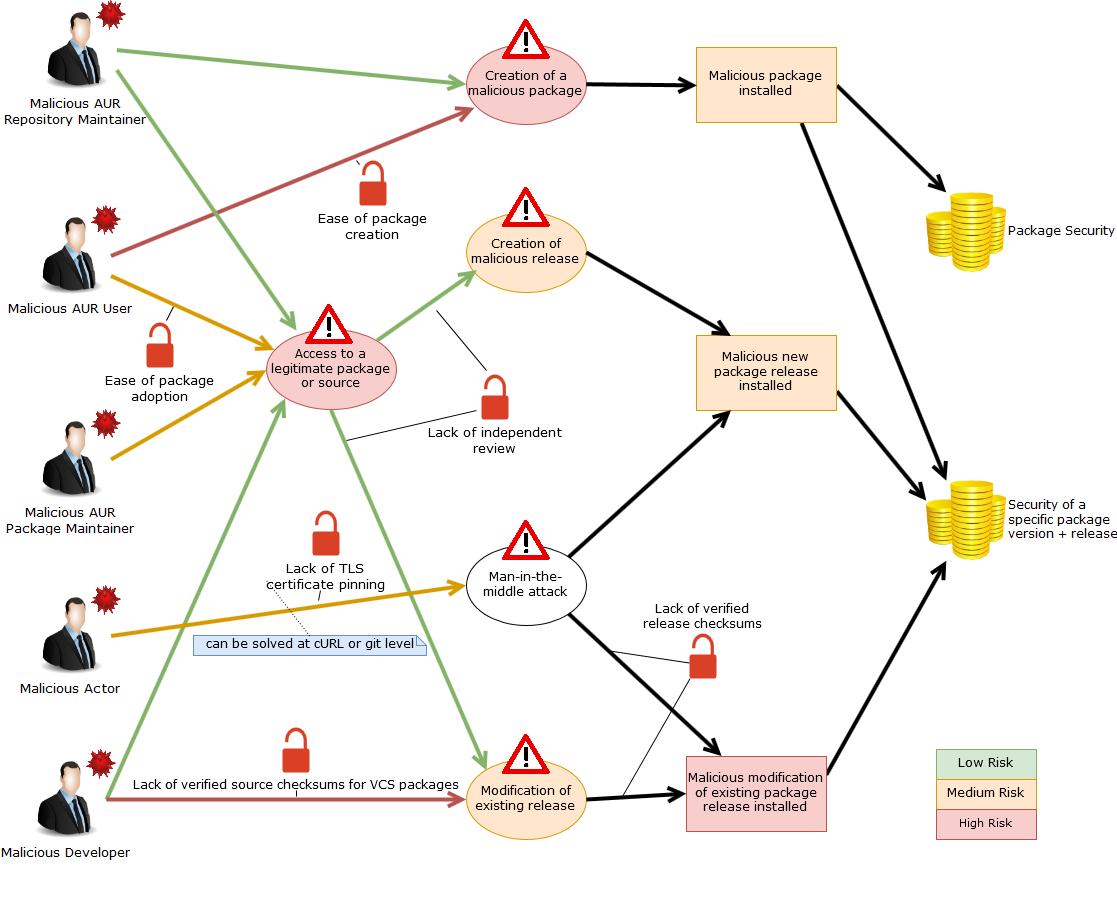
\includegraphics[width=\textwidth]{threat1n}
	\caption[Threat Assessment]{Threat Assessment of the Arch User Repository}
	\label{fig:threat}
\end{figure}
\end{center}

\subsection{Concrete Attack Scenarios}
\label{sec:attack_scenarios}
We used the CORAS \cite{Dahl:2007} threat modeling language to arrange the security issues in such a way that concrete attack scenarios are intuitive to comprehend and retrace. The resulting threat diagram can be seen in Figure~\ref{fig:threat}.

Many of the AUR's security issues, which emerged out of its design, are not easily solvable and are only included for completeness. However, Figure~\ref{fig:threat} shows that the vulnerabilities converge inwards and meet in only three points; This means that security issues further along the right of the diagram tend to be more promising candidates in the search for solvable problems.

This knowledge leads to two concrete attack scenarios that could be preempted without redesigning the AUR. These are outlined below.

% Threats:
\subsubsection{Tampered VCS Sources: Malicious Upstream}
\label{sec:vcs_attack}
In some cases, the user is not adequately protected against malicious (or compromised) upstreams:
The AUR supports so-called \emph{VCS packages} \cite{wiki:VCSPackages}, which download sources from a version control system, such as Git or Mercurial, instead of downloading a fixed archive. This relieves maintainers from updating their \texttt{PKGBUILD} for every new commit.
\texttt{makepkg} will even automatically calculate the up-to-date version number using for instance tags and commit numbers.

VCS packages were primarily designed to simplify the installation of up-to-date packages from source, and they do that well; however they also introduce a security issue:
Since the \texttt{PKGBUILD} does not need to be updated between versions, it cannot contain checksums for the new version either.
This used to be thought a small issue since most modern version-control systems use cryptographic hash functions for commit identification and integrity verification.
However, all popular ones use SHA-1, which has already been broken \cite{Stevens:2017}.
This means that attacks on VCS repositories using hash collision are possible.
In that light, users don't have a way to verify the authenticity of the source which they are downloading while building a VCS package, unless they can trust the upstream itself, meaning that no-one will notice if the upstream is compromised or makes malicious changes.
There is no way to counter this except to manually audit the upstream sources, which \emph{should} primarily be the maintainer's responsibility.

\subsubsection{Tampered Packages: Malicious Maintainer}
\label{sec:maint_attack}
Users are also not adequately protected against malicious maintainers:

Because it is easy to gain access to a package, e.g. by adopting an orphan or simply by creating it, and nothing is verified or audited before publication, it is easy for a malicious agent to modify a package.
Additionally, since the \texttt{PKGBUILD} is not signed or hashed, users will not notice if the build instructions for a specific package version were modified. This allows targeted attacks:

If the time at which targets will update their machine is known and one has access to an AUR package which they expected to update, malicious code can be introduced into the corresponding \texttt{PKGBUILD} or \texttt{.install} files within that update window.
This could be as simple as changing the checksum if one also has access to the upstream source code (even a very careful user has no chance of noticing this attack), or executing innocuous code in the install file or \texttt{PKGBUILD} itself.

The malicious change could be reverted immediately afterwards. If the time frame is short, no other AUR user (and thus, \emph{no-one}) would ever notice.
One can only defend against this with a good local trust model, such as that possible with \texttt{bauerbill}, or manual cryptographic verification of the git commit to the AUR, if the attack was conducted by adopting an orphan package --- assuming that the maintainer signs his commits, which is only rarely the case.
 % BENNETT

  \section{AURsec}
    % TODO: maybe main tool - aursec; initialization - aursec-init; API - aursec-chain
    \label{sec:AURsec}
\begin{figure}
	\centering
	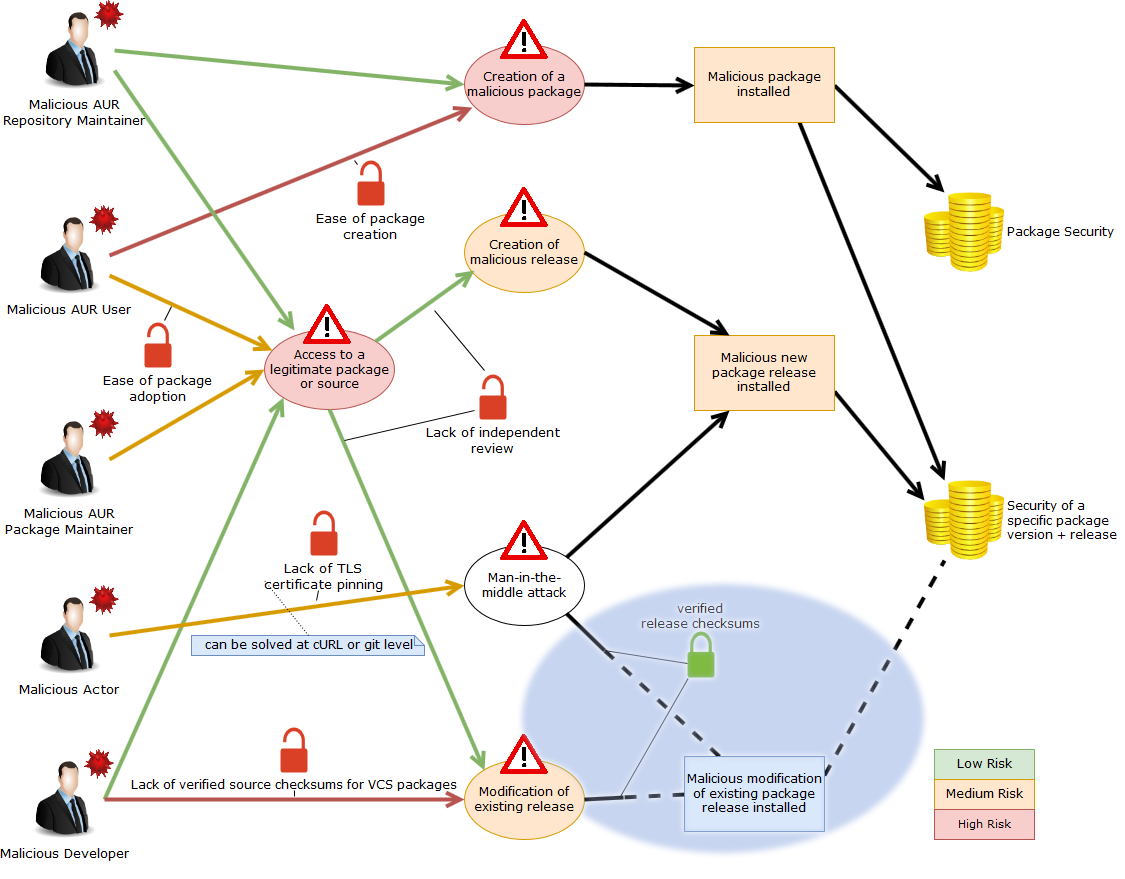
\includegraphics[width=\textwidth]{threat2n}
	\caption[Threat Prevention Strategy]{Strategy for Improving the Security of the AUR}
	\label{fig:threat2}
\end{figure}

Defence against the two attack scenarios mentioned in Section \ref{sec:attack_scenarios} requires the availability of cryptographically secure release hashes for every version of every package (Figure \ref{fig:threat2}).
If those were available, an attack would result in a hash mismatch and therefore the user could be warned.
However, the focus of the AURs design on simplicity, automation and fast package updates prevents any secure implementation on the server side as it would require the introduction of a central point of trust. That trust could only be maintained through the introduction of manual auditing, which is the opposite of what the AUR was designed for.

The solution must therefore be to implement a (preferably distributed) database on the user side, which means that there is no single authoritative source.
Since the aim is to defend against \emph{targeted} attacks, the assumption being that only comparatively few users will encounter a malicious version, this can be circumnavigated by checking the hash against a \emph{consensus} formed by many users.

% TODO: @important @lukas @bennett This paragraph is probably still unclear... need to think about that!
To make the database as safe as possible, a blockchain is used. The chain contains a smart contract providing securely callable functions. With one of these functions it is possible to commit a hash for a specific package and version.
This hash will be saved in the blockchain only if this user has not committed the same hash before, thereby making it harder to take over the blockchain and get a malicious hash to be the consensus.
The consensus is updated after every hash commit. Another function is used to get the current consensus hash and its valid commit count for a specific package and version.

This is the first project to use a blockchain as a means to provide distributed verification of (software) downloads.

% Workflow
\subsection{Workflow}
\label{sec:workflow}
The following workflow is visualized in Figure \ref{fig:main_workflow}.
\begin{figure}[!htb]
	\centering
		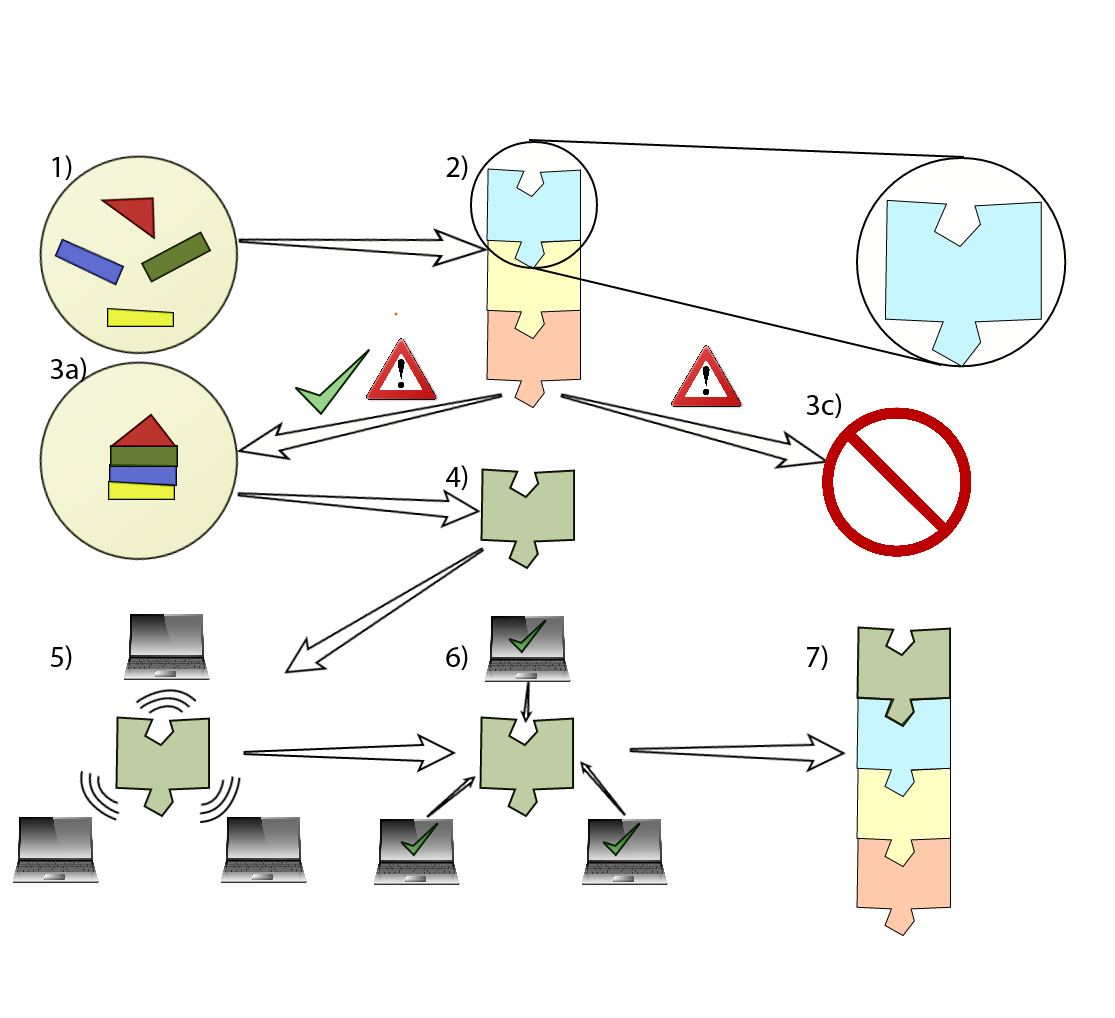
\includegraphics[width=0.6\paperwidth]{Workflow2}
	\caption{Main (Blockchain) Workflow}
	\label{fig:main_workflow}
\end{figure}

\begin{figure}[!htb]
	\centering
		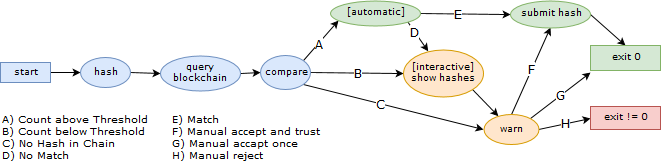
\includegraphics[width=\textwidth]{decision2}
	\caption{Aursec State Machine}
	\label{fig:state_machine}
\end{figure}


First of all a \texttt{PKGBUILD} is downloaded and partially executed in a sandbox in order to get the package version and download VCS sources (1).
Then, it is hashed along with any VCS sources and \texttt{.install} files.
The resulting local hash is compared with the current consensus (most often committed) hash of this package-version on the blockchain (2).

Depending on the comparison of the hashes (3), one of three things will happen [Figure~\ref{fig:state_machine}]:
The package may be created, installed and the hash will be added to the blockchain \emph{(Followed by step 4)} if the hashes match and the number of commits is above the trust threshold or the user decides to trust the locally generated hash anyway (A, F).

The package may be created and installed but the hash will not be added to the blockchain if the hashes do not match and/or the number is below the threshold, but the user wants to create and install the package without committing the hash. In this case the program exits with a zero status (B \rightarrow~G).

The package may not be created and installed because the hashes do not match and/or the number is below the threshold and the user doesn't want to create the package. In this case the program exits with a non-zero status (H).

If the locally generated hash is trusted, the local hash is committed to the blockchain (4). This is a transaction [see \texttt{aursec-chain commit-hash)}].
All nodes in the blockchain get the transaction over the network (5) and the transaction will be verified (together with all other transactions since the last block) and included the next mined block (6).
This mined block is then added to the blockchain (7).
As the transaction is included in a mined block, the consensus is atomically updated to reflect the new hash submission.
 %LUKAS
    \subsection{Blockchain implementation}\label{sec:aur-block}
In our approach we used Ethereum as blockchain and Solidity as the programming language for the smart contract.
We have chosen Ethereum because our blockchain has to fulfill several requirements:

Since we target Arch Linux, it must be easy to install on this platform.
This is covered by the \emph{geth} package which is available in the official community repository and can be directly installed using pacman.
The blockchain also needs to provide an API which allows external scripts to work with it.

Ethereum provides two APIs:
An IPC (interprocess communication) API, which allows connecting an interactive \emph{geth} console to a running blockchain, but is not convenient for external scripts,
and an HTTP RPC (remote procedure call) API which allows to send HTTP requests containing JSON bodies.
These requests can be sent with external scripts and programs since nearly every programming and scripting language (including bash) has HTTP support.
In our approach the shell script \texttt{aursec-chain}~(Section~\ref{sec:aursec-chain}) and the Python script \texttt{aursec-tui}~(Section~\ref{sec:tui}) use this API to interact with the blockchain.

The blockchain also needs to support smart contracts in order to allow us to use the blockchain functionally.
Ethereum not only supports smart contracts, they are it's main feature.
The specially developed high-level language \emph{Solidity} allows to write smart contracts in little time.

Our smart contract (Appendix~\ref{sec:contract}) provides two public functions which allow users to submit hashes (line 56) and to request the current consensus hash of a versioned package (line 43).
The contract allows each user to commit a hash only once: further commits of the same hash by the same user will not be considered in order to prevent manipulation of the consensus. This is implemented by keeping track of who submitted a hash (lines 58-60).

Finally, the blockchain needs to to provide an easy way to create private networks separate from the main one.
It would be safer to use the main blockchain because larger chains are harder to manipulate, and miners would get currency worth real money (in addition to secure software downloads) for their work, but we decided against that because the main blockchain takes up a lot of disk space and has much higher mining costs than makes sense for our application.
Ethereum provides possibilities to create private networks easily; It is only required to choose a network ID and to host the bootnode that is required to build the peer to peer network.
Our bootnode is active 24/7 on a DigitalOcean droplet provided by our supervisor.
Appendix \ref{sec:init-boot} explains how a new bootnode is added to the aursec-network.
 % LUKAS
    \subsection{Initialization - aursec-init}\label{sec:aursec-init}
Aursec-init is a shell script which allows the user to create all requirements for using our project.
It can also be used to rebuild the local copy of the blockchain, effectively re-installing from scratch.

First, it creates all needed folders and markers.
These markers track when hash commits and mining take place and are used by the systemd-service \textit{aursec-blockchain-mine} to adjust the mining effort based on recent hash commits.
Then, it creates the blockchain from our \emph{genesis block}, which is the first block in the blockchain.
After that, the synchronization of the blockchain begins.
In the meantime, the generation of the first two \emph{Directed Acyclic Graphs} (DAG) is stated.
Every DAG is a \~1GB dataset which is needed for mining new blocks \cite{wiki:DAG}.
Finally, the script mines a few blocks to gain enough currency to enable committing of hashes right after the initialization.
 % LUKAS
    \documentclass[11pt]{scrartcl}

%\usepackage[utf8]{inputenc} % use UTF-8 as input encoding - not necessary with xelatex
%\renewcommand{\baselinestretch}{2} % Line height
\usepackage[T1]{fontenc} % make non-ASCII characters cut&pastable in PDF
\usepackage{lmodern} % easiest way to get outline fonts with T1 encoding
\usepackage[english=american]{csquotes} % automatic quotation style
\usepackage[american]{babel}
\usepackage{abstract}

\usepackage{amsmath,amssymb} % math
\usepackage{caption} % For caption*
\usepackage[hidelinks, colorlinks=true]{hyperref} % Make links from things

\usepackage{graphicx} % images
\DeclareGraphicsExtensions{.eps,.pdf,.png,.jpg,.gif}
\graphicspath{{./img/}}
\usepackage{tabularx} % tabulars
\usepackage{array,booktabs} % rules for frontpage
\usepackage{titling} % "vars" for titlepage
\usepackage{minted} % syntax highlighting
\usepackage{csquotes} % display quotes
\usepackage{cleveref}
\usepackage{framed}
\usepackage{array}
\newcolumntype{L}[1]{>{\raggedright\let\newline\\\arraybackslash\hspace{0pt}}m{#1}}
\newcolumntype{C}[1]{>{\centering\let\newline\\\arraybackslash\hspace{0pt}}m{#1}}
\newcolumntype{R}[1]{>{\raggedleft\let\newline\\\arraybackslash\hspace{0pt}}m{#1}}


% Setup the page geometry
\usepackage[a4paper,top=3cm,bottom=3cm,left=3cm,right=3cm]{geometry}
%\usepackage[a4paper,margin=5cm,top=3cm,bottom=3cm,left=2.7cm,right=2.7cm]{geometry}



\title{AURsec}
\newcommand{\titlesub}{Detecting and preventing targeted attacks in the Arch User Repository: A~blockchain-based~approach}
\author{Bennett Piater \& Lukas Krismer}
\newcommand{\leader}{Supervisor: Christian Sillaber}
\newcommand{\university}{University of Innsbruck}
\newcommand{\course}{Bachelor thesis}
\date{\today}

\begin{document}
  %%% Boilerplate
  \thispagestyle{empty}

  %frontpage
  \begin{titlepage}
    \noindent
    \begin{tabular}{@{}p{\textwidth}@{}}
        \toprule[2pt]
        \midrule
        \vspace{0.15cm}
        \begin{center}
            \Huge{\textbf{\thetitle}} \\
            \normalsize{\titlesub}
        \end{center}
        \vspace{0.15cm}\\
        \midrule
        \toprule[2pt]
    \end{tabular}
    \vspace{4 cm}
    \begin{center}
        \vspace{0.2cm}
        \LARGE{\theauthor} \\
        \vspace{0.1cm}
        %{\small \matrikel}
    \end{center}
    \vfill
    \begin{center}
        \course \\
        %\group \\
        \leader \\
        \vspace{1.2 cm}
        \university
    \end{center}
\end{titlepage}

  %  \vspace*{\fill}
\thispagestyle{empty}
  \begin{center} \textbf{\large{STATUTORY DECLARATION}} \end{center}
  I declare that I have authored this thesis independently, that I have not used other than the declared sources  /  resources,  and  that  I  have  explicitly  marked  all  material  which  has  been  quoted  either literally or by content from the used sources.

  \begin{center}
  \begin{table}[!htb]
  \begin{tabularx}{\textwidth}{lXX}
  Innsbruck 17.05.2017 & \_\_\_\_\_\_\_\_\_\_\_\_\_\_\_\_\_\_ & \_\_\_\_\_\_\_\_\_\_\_\_\_\_\_\_\_\_ \\
  Location,Date & Bennett Piater & Lukas Krismer \\

  \end{tabularx}
  \end{table}
  \end{center}
  \vspace*{\fill}
  \pagebreak 
f


  \pagenumbering{Roman}
  \begin{abstract}
    The Arch Linux User Repository is fundamentally insecure.
It was designed for simplicity and rapid iteration, leaving its users unprotected against many kinds of attacks.

This project increases its security by:
\begin{enumerate}
	\item Analyzing its security issues
	\item Creating a threat model
	\item Solving one of these issues, the \emph{lack of verified release checksums}, thereby protecting users against targeted attacks and compromised sources.
\end{enumerate}

For this purpose we compare the downloaded package sources with the hashes submitted by other users in a secure database where every user is allowed to upload each hash only once.
The database of choice was a blockchain capable of smart contracts because it is distributed and fulfills our security requirements.

  \end{abstract}

  \section*{Foreword}
  This thesis is written as part of the completion of the Bachelor of Computer Science (``Informatik'') by Bennett Piater and Lukas Krismer.

We chose this topic because we already used Arch Linux including the AUR and are generally interested in security. As users of the AUR we wanted to make it more secure, not only for us, but for all users.

\paragraph*{}

We want to thank Christian Sillaber for his supervision and
and our families and friends for their support.
We want to specially thank Justus Piater for his comments on how to improve the structure of the paper, Sara Bauer for her correction of our use of the English language, and Alad Wenter for his help during the integration with the AUR helper \texttt{aurutils}.

  \pagebreak


  \tableofcontents
  \listoffigures
  % \listoftables
  \pagebreak


  %%% Content starts here
  \pagenumbering{arabic}

  \section{Introduction}  %(1/2 page)
    \label{sec:intro}
The Arch Linux distribution constitutes a simple infrastructure which makes it easy to customize and participate in its development. As such, it provides packaging tools that facilitate the creation of custom packages and has attracted a very active community.
These facts necessitated the establishment of a place where active users could make their own packages available for others to use.

To address this issue, \texttt{ftp://ftp.archlinux.org/income} was created as a staging area; packages could be stored there until official maintainers would adopted them. However, waiting for the maintainers' participation implied a certain delay, so another solution was needed.
The next improvement constituted the \emph{Trusted User Repositories}, in which some privileged users, many more than the maintainers, were allowed to host their own repositories for anyone to use.

To completely remove the delay the \emph{Arch User Repository} (AUR) was created. The custom repositories were consolidated into one single repository, and the requirement to be a \emph{Trusted User} was dropped.
Thanks to the removal of all middlemen, everyone can now upload their packages to one central location. \cite{wiki:AUR}

The AUR is similar in design to PyPI (for Python), NPM (for Javascript) and rubygems.org, where all users can share their packages. All 4 platforms share a focus on simplicity, ease of use, and rapid iteration (creation of packages and roll-out of updates) at the expense of security.
The desire to allow anyone to use the system and to push out updates rapidly makes it hard to include proper vetting of contributors or auditing of software, thereby enlarging the possibility attacks.

\subsection*{Improving the Security of the AUR}
Most of the AUR's security issues are inherent to its design and thus cannot be solved without changing the AUR's concept in its entirety.
Nevertheless, some of them, which make users susceptible to targeted attacks through manipulated packages, can be remedied without modifying the AUR directly. That is the purpose of this paper.

Since targeted attacks only affect a small percentage of total users, they could be prevented by performing an additional integrity check which raises alarm if someone receives a different package than the majority of users.

This solution approach requires a tamper-proof, trust-less, preferably distributed database through which the most-seen hashes of a package can be tracked. Blockchains are a possible choice, as they fulfill all of these requirements.
Our tool \emph{aursec} hashes per-package information from the AUR and compares it to the most submitted hash of the corresponding package version stored in an Ethereum blockchain.
If the hashes differ, the user is warned of a possible attack.


% TODO: @important quick structure introduction?
% NOTE: I would ask christian
% Maybe ~one sentence about each section...

% Section 2 introduces blockchains, why we use one and why we chose Ethereum specifically.
% Section 3 is a threat assessment of the AUR including two concrete attack scenarios against which we want to defend.
% Section 4 describes our solution and implementation in detail.
% Section 5 lists some of the things we learned while working on our solution which may be of interest to readers.
% Section 6 discusses inherent qualities of our approach and compares it to other possible approaches.
% Section 7 evaluates our work by demonstrating how well we solved the problem that we set out to solve as well as discussing its usability and sensibility according to our experience and feedback from users.


  \section{Related Work}
    \label{sec:related}
\subsection{Arch}
Arch Linux \cite{wiki:arch} is a lightweight GNU/Linux distribution.
It was created by the Canadian Judd Vinet between 2001 and 2002 and further developed until today.
The renowned Arch Wiki was created in 2005. Since 2007 Aaron Griffin leads the development, which is completely done by part time volunteers in order to remain free from corporate influence.

Arch Linux follows the rolling-release model instead of periodical releases to provide the users the newest possible stable version of every program.
Upstream software is modified as little as possible and only as much as needed to integrate with the rest of the distribution.

Arch makes many features available earlier than other distributions, such as the systemd init system, software raids and new file systems.
Systemd \cite{wiki:systemd} replaced the \emph{System V init system} in 2013 \footnote{\url{https://bbs.archlinux.org/viewtopic.php?pid=1149530\#p1149530} accessed June 2, 2017}.
It provides a system- and service manager which starts the rest of the system and manages daemons and background services.
Systemd services are easy to handle and to configure.

Arch provides open-source packages as well as proprietary software to let the user decide if he wants functionality or if he wants to stay with the open-source ideology when they conflict.
Users can install them with the lightweight package manager \texttt{pacman}, which is one of the core tools of Arch.
Pacman uses a simple binary package format and an easy-to-use build system. It allows to manage the packages from the official repositories as well personal builds.

Arch is a lightweight distribution, which means that the user has to install and configure everything himself.
Arch does not want to be user-friendly, but rather user-centric.
This is achieved by providing the user with many possibilities to create his own personalized system and help him fix issues himself.
Arch encourages tinkering and caters to power users who want to understand and configure much of their system.
There are mailing-lists, an official Wiki, an official Forum, a bug tracker and several other places where users can get help.
Most members of the community are experienced Linux users who are willing to read documentations and solve problems on their own with the help of the community, as well as help others.

It is notoriously hard to estimate the popularity of Linux distributions, and so it is hard to tell how wide-spread Arch Linux is.
Arch users can voluntarily submit a list of their installed packages for statistical evaluation by installing and calling a script called \texttt{pkgstats}.
These stats show 13,353 different IP addresses from Arch users as of June 12, 2017~\cite{arch:stats}, which is fairly small.
However, no one knows how to control for administrators using many Arch machines behind one router, which seems to be common, and for the (probably many) users who do not submit these statistics.
According to the results of the yearly Reddit Linux Distribution Survey on \texttt{/r/linux} in 2015, 28.47\% of the participating users used Arch Linux~\cite{linuxsurvey}, with only Ubuntu appearing in the same order of magnitude.
Overall, it seems that Arch is a small, but very active distribution with comparatively vocal users. It's popularity has been steadily increasing for the past few years.

\subsubsection{AUR}
The Arch User Repository (AUR) is an unofficial, community-driven repository for Arch users.
It contains \texttt{PKGBUILD}s which are package descriptions containing all information needed to create packages from source using a tool called \texttt{makepkg}.
These packages can then be installed with \texttt{pacman}, Arches normal package manager.
Everyone can upload packages to the AUR as well as download them.
The uploaded packages are not verified or audited in any way in order to minimize the delay between the upload and the availability of a version.
Users can vote for packages; Packages with enough votes may get adopted by a maintainer and moved to the official Arch community repository.
If all maintainers of a package no longer want to maintain it, it can be orphaned. Any AUR user may adopt orphan packages.
\cite{wiki:AUR}

\subsection{Blockchain}\label{sec:ABCblockchain}
A blockchain is similar to a distributed database system which is not owned by a single user.
The first blockchain was implemented by Santoshi Nakamoto in 2008.
This blockchain is based on research of the early 1990s where the concept of cryptographically secured blocks was first described.
It is also the core of the bitcoin currency.
Since then several blockchain approaches where deployed.

As opposed to classic databases, blockchains maintain the entire transaction history.
Every user can look into this history and can track other users because the transactions are not anonymous.
Because of that, blockchains are the first digital approach of decentral database solving the double-spending problem.

Normally blockchain networks are peer-to-peer.
If a user wants to add a transaction to the blockchain, the transaction is encrypted, sent to all users, and verified.
If the majority of users validates the transaction, the data is added to the blockchain in the next block.
Underwood describes these transactions as ``... secure, trusted, auditable, and immutable''~\cite{Underwood}, which means that the transactions cannot be manipulated without a majority consent.

Users do not trust the result of a single node, but that of the majority.
As a result, blockchains are highly ``Byzantine''-fault tolerant.
This means that attackers need more than 50\% of the computation power to manipulate a blockchain (because then the attacker can produce more blocks than the rest).
If attackers gets more than 50\% of the computing power, they can manipulate the chain because the longest chain is always considered the canonical one.
Shorter tails become orphans and are rejected by the network.

Because blockchains are distributed and every user has a synchronized copy of the chain (which often requires several GB of disk space), they do not have a single point of failure or require backups.
The benefits of a blockchain compared to a conventional database are: (a) The blockchain can be directly shared because transactions contain their own proof as provided by a sophisticated cryptographic algorithm. (b) The blockchain is more robust (even than distributed databases).
Blockchains are often used to store transactions of concurrency (e.g. bitcoin), identity management or medical records.
\cite{Underwood,blockchain:eco}\newline\newline

To create new blocks \textbf{miners} are needed (proof of work).
A miner is the computer which has found a hash since the last block based on the transaction information and other data such as the hash of the last block.
This hash has to fulfill several requirements; The more there are, the more the mining difficulty increases.
It is hard to find a hash but it is easy to check if the hash fulfills all the requirements.
This is important because it makes it possible for every node to verify every block.

The mining difficulty describes the time effort required for mining of a block.
If the mining difficulty is high, the miner receives more \emph{coins} (Ethereum uses \emph{ether}) to reward the effort.
Coins are needed to perform transactions.
However, the effort and the payment have to be in sound relation to one another: that is, the miner's effort must not deceed or exceed the payment.
If the mining difficulty is too high in relation to the reward, it can lead to less blocks per hour which by implication leads to high transaction latencies because the transactions are not validated for considerable time.
If the opposite happens, there will be a low transaction per block ratio which makes the blockchain unnecessarily big; Users could also flood the chain with very many transactions, weakening the meaning of majority consent.\newline\newline

To provide functionality extending the transaction of coins, the blockchain has to accept \textbf{smart contracts}.
Smart contracts use computerized transaction protocols to execute the terms of a contract which are agreed upon by the users.
The term \emph{Smart Contract} might be misleading, as in reality it is a sequence of handling arrangements which map the contract clauses into code \cite{ecolex} --- they are effectively \emph{functions} of which the semantics may not be changed after all parties agreed on them.
Smart Contracts defining rules, penalties around an agreement and automatically check and impose them.

Without smart contracts, a blockchain can only handle the transaction of coins.
With smart contracts, a blockchain can be used as a database, containing objects which can be created, modified and deleted by \enquote{intelligent} transactions.
Additionally, object properties may be read without performing a transaction, allowing users to read information without paying currency.
The functions requiring coins are executed by every miner and are ACID transactions (atomic, consistent, isolated, durable).
Since the contract code is included in the chain, it is guaranteed to be immutable and therefore impossible to manipulate.
This guarantees that one is able to run secure code on the blockchain.

By avoiding middleman (e.g. lawyers), smart contracts are safer and often cheaper than their real-world counterpart.
They are safer because all parties communicate directly, and cheaper because the transaction fee is normally cheaper than the costs of a lawyer or notary.
Smart contracts can be used in different systems:
The Governments could use them for electronic voting systems, Companies already use them (e.g. Ethereum \footnote{\url{https://entethalliance.org/}) accessed on June 20, 2017}) in different ways and they are also used in healthcare systems (e.g. gem \footnote{\url{https://gem.co/} accessed on June 20, 2017}) which store the data in the blockchain and make it available for authorized users (e.g. doctors).
The healthcare-example also shows another advantage of smart contracts.
People cannot ``lose'' their data because its in the blockchain which is distributed.
Also Smart Contracts are more accurate than manually filled forms because they avoid manual errors.

Blockgeeks explains Smart Contracts with the following example:

\begin{displayquote}
	Suppose you rent an apartment from me. You can do this through the blockchain by paying in cryptocurrency. You get a receipt which is held in our virtual contract; I give you the digital entry key which comes to you by a specified date. If the key doesn’t come on time, the blockchain releases a refund. If I send the key before the rental date, the function holds it releasing both the fee and key to you and me respectively when the date arrives. The system works on the If-Then premise and is witnessed by hundreds of people, so you can expect a faultless delivery. If I give you the key, I’m sure to be paid. If you send a certain amount in bitcoins, you receive the key. The document is automatically canceled after the time, and the code cannot be interfered by either of us without the other knowing, since all participants are simultaneously alerted.~\cite{blockgeeks}
\end{displayquote}

Finally, one must mention that smart contracts are not perfect. Bugs in the code can lead to vulnerabilities which can be used to attack a blockchain.
The most popular example for this case is the ethereum-hard-split in 2016 \cite{heise-dao} where a bug in a smart contract was used to attack the Ethereum blockchain and steal 3,6 million ether-coins.
Furthermore, misunderstandings in traditional contracts can be fought over in court, but smart contracts cannot be modified or prevented from executing.
\cite{blockgeeks}


\subsection{Ethereum}
Ethereum is a blockchain-based, open-source, distributed computing platform developed by Vitalik Buterin, Gavin Wood and Jeffrey Wilcke.
It provides smart contract functionality. These smart contracts are usually written in the specially developed, Turing-complete language \emph{Solitidy}.
Solitidys syntax is similar to the syntax of JavaScript.
Every node runs an instance of the \emph{Ethereum Virtual Machine} (EVM), which can execute code of arbitrary complexity; The smart contracts are executed on the EVM.
Every EVM in the network executes the same instructions.

Ethereum rewards mining effort with it's currency, ether-coins.
As of June 3, 2017, the blockchains holds 92,2 Million Coins and is worth more than 20 billion US\$, which makes it the second most valuable blockchain after Bitcoin.
While every transaction in bitcoin costs exactly the same, transactions in ethereum have different fees based on the required storage, code complexity and bandwidth usage of smart contracts they interact with.
Beside it's main blockchain, Ethereum provides all the required infrastructure to create private blockchains.
\cite{ethereum, wiki:ethereum}

Bloomberg \cite{bloomberg:eth} describes Ethereum as \enquote{shared software that can be used by all but is tamperproof. You can safely do business with someone you don’t know, because terms are spelled out in a \enquote{smart contract} embedded in the blockchain. There could be blockchain versions of Uber and Airbnb that are peer-to-peer: No company would need to sit in the middle of the transaction to gather data about your spending habits or collect a fee.} %\cite{bloomberg:eth}


    \subsection{Other Approaches}
\emph{AUR helpers} have been developed to make the usage of the AUR easier.
They are designed to assist users with installing and updating packages from the AUR by automating some or all of the workflow (A detailed comparison can be found in the Arch Wiki~\cite{wiki:aur-helper}).
Some of them also give some degree of additional security compared to fully manual building.
In this section we want to look at \emph{yaourt}, \emph{bauerbill} and \emph{aurutils}.

Yaourt is the most popular AUR helper, but it is also one of the most insecure approaches~\cite{wiki:aur-helper}.
The user can use a command-line parameter to skip the only security layer, the manual \texttt{PKGBUILD}-check.
Users of Bauerbill and aurutils always have to check their \texttt{PKGBUILD}s.
Furthermore, aurutils makes the manual verification of \texttt{PKGBUILD}s easier by creating \emph{diffs} which show the changes between the last installed version and the current \texttt{PKGBUILD}.
Aurutils does not install the packages directly using pacman;
Instead, it adds or updates the package into a local repository.
These packages can be cryptographically signed by the user to ensure that they cannot be manipulated after they were created.
Pacman can then access this repository and install packages from it like from the official ones.
Bauerbill directly installs the packages after the \texttt{PKGBUILD}-check using pacman, but it displays if the maintainer of a package has changed since the last update.


  \section{Motivation: Security Issues of the AUR} %(1 1/2 pages)
    \label{sec:security_issues}
    \label{sec:motivation}
Ease of use appears to have been, if not the only, at least the primary design consideration of the Arch User Repository. This creates so many security issues that it is actually quite a task to address them all.

% PKGBUILDS
\subsection{Local Package Creation}
One of the most obvious problems is the installation procedure itself.
Arch packages are created locally from a bash file, the so-called \texttt{PKGBUILD} \cite{wiki:PKGBUILD}, containing metadata such as name and version, the URLs and checksums of upstream sources, and functions for the compilation and packaging steps.

The AUR contains these \texttt{PKGBUILD}s and possible patches to be applied to the upstream sources in a git repository per package.
A package file can be produced by cloning its repository and using a tool called \texttt{makepkg} \cite{wiki:PackageCreation}, which sources the script, downloads and verifies the sources, and calls the compilation and packaging functions.

This means that users can verify what they are compiling as opposed to blindly trusting binaries created by third parties; however, it also means that the maintainers of AUR packages have a means of executing arbitrary shell commands on users' machines.

This is aggravated by the fact that \texttt{PKGBUILD}s can include a \texttt{.install} file into the built package, which will be executed \emph{as root} when the package is actually installed.
The risk increases further if \emph{AUR helpers} are used, because some of them are unsafe in that they execute code before giving users the opportunity to inspect it, or disincentivize them from doing so.

\subsection{The Trust Issue}
Another problem is that users are not given any reason to trust the maintainers.
Unlike the official repositories, where maintainers are vetted, packages are (often manually) audited before being accepted, and everything must be signed with a trusted OpenPGP key, anyone can create an account and submit a new package to the AUR in a few minutes.
There is no admission procedure or audit system and no OpenPGP web of trust in order to minimize the time needed to publish a package or update.

\texttt{makepkg} can verify OpenPGP signatures for upstream sources, but the \texttt{PKGBUILD} itself could only be signed by using signed git commits, which is unfortunately not enforced or even officially recommended --- and not supported by any AUR helper anyway.

Except when using the AUR helper \texttt{bauerbill} \cite{bauerbill}, which provides a basic user-side trust management system (see Section~\ref{sec:security_comparison}), the only way to be maintain reasonable trust is to manually read every single file, which is cumbersome.
Since only security-conscious users are willing to put in so much effort before trusting a \texttt{PKGBUILD}, most users are left vulnerable.

\subsection{Adopting orphan packages}
The trust issue is aggravated by the fact that packages can silently and quickly be taken over by other maintainers due to the orphan/adoption system.

When maintainers want to stop maintaining a package, but the package is still useful and actively developed upstream, they have the option to \emph{orphan} it rather than deleting it.
Orphan packages can be \emph{adopted} by any AUR user, at any time, without delay.
This feature was designed to minimize update delay, which it does effectively; however, it also makes it easy for malicious agents to take over popular orphaned packages, manipulate them, and immediately orphan them afterwards.

\begin{center}
\begin{figure}
	\centering
	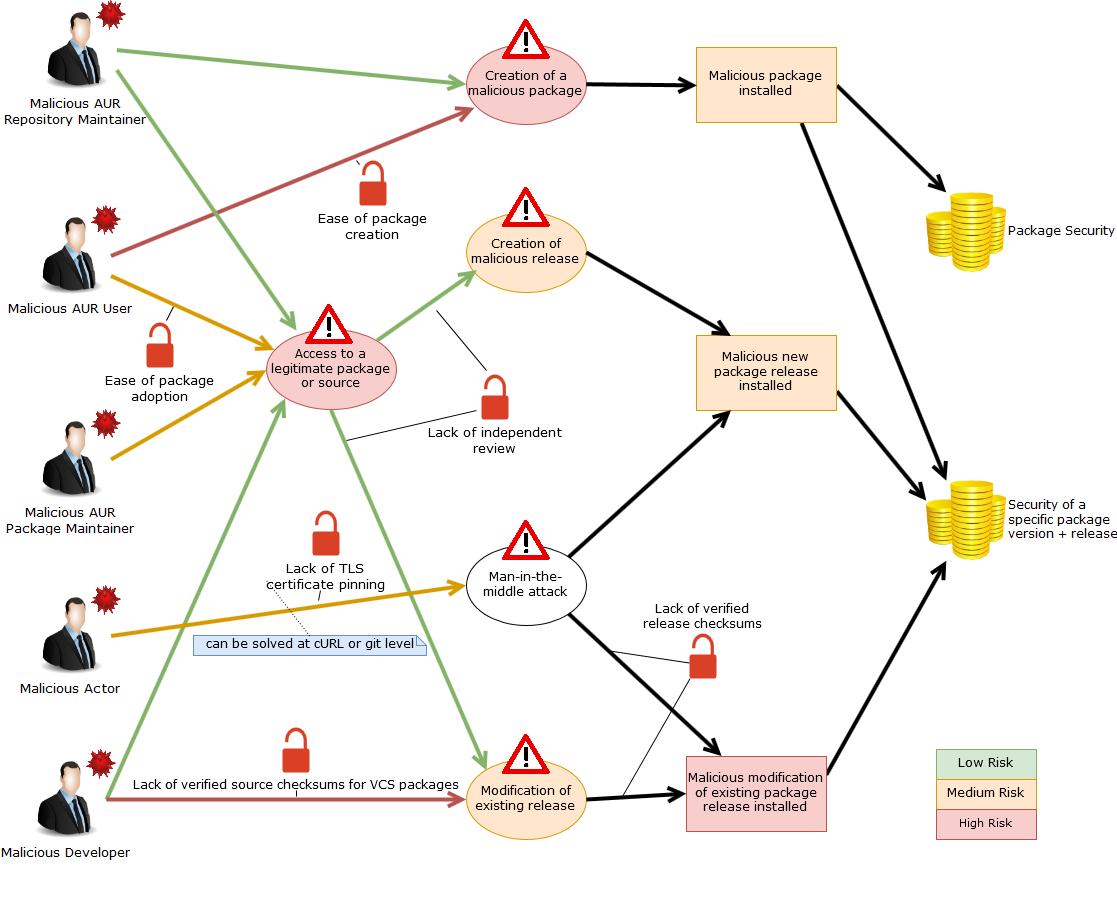
\includegraphics[width=\textwidth]{threat1n}
	\caption[Threat Assessment]{Threat Assessment of the Arch User Repository}
	\label{fig:threat}
\end{figure}
\end{center}

\subsection{Concrete Attack Scenarios}
\label{sec:attack_scenarios}
We used the CORAS \cite{Dahl:2007} threat modeling language to arrange the security issues in such a way that concrete attack scenarios are intuitive to comprehend and retrace. The resulting threat diagram can be seen in Figure~\ref{fig:threat}.

Many of the AUR's security issues, which emerged out of its design, are not easily solvable and are only included for completeness. However, Figure~\ref{fig:threat} shows that the vulnerabilities converge inwards and meet in only three points; This means that security issues further along the right of the diagram tend to be more promising candidates in the search for solvable problems.

This knowledge leads to two concrete attack scenarios that could be preempted without redesigning the AUR. These are outlined below.

% Threats:
\subsubsection{Tampered VCS Sources: Malicious Upstream}
\label{sec:vcs_attack}
In some cases, the user is not adequately protected against malicious (or compromised) upstreams:
The AUR supports so-called \emph{VCS packages} \cite{wiki:VCSPackages}, which download sources from a version control system, such as Git or Mercurial, instead of downloading a fixed archive. This relieves maintainers from updating their \texttt{PKGBUILD} for every new commit.
\texttt{makepkg} will even automatically calculate the up-to-date version number using for instance tags and commit numbers.

VCS packages were primarily designed to simplify the installation of up-to-date packages from source, and they do that well; however they also introduce a security issue:
Since the \texttt{PKGBUILD} does not need to be updated between versions, it cannot contain checksums for the new version either.
This used to be thought a small issue since most modern version-control systems use cryptographic hash functions for commit identification and integrity verification.
However, all popular ones use SHA-1, which has already been broken \cite{Stevens:2017}.
This means that attacks on VCS repositories using hash collision are possible.
In that light, users don't have a way to verify the authenticity of the source which they are downloading while building a VCS package, unless they can trust the upstream itself, meaning that no-one will notice if the upstream is compromised or makes malicious changes.
There is no way to counter this except to manually audit the upstream sources, which \emph{should} primarily be the maintainer's responsibility.

\subsubsection{Tampered Packages: Malicious Maintainer}
\label{sec:maint_attack}
Users are also not adequately protected against malicious maintainers:

Because it is easy to gain access to a package, e.g. by adopting an orphan or simply by creating it, and nothing is verified or audited before publication, it is easy for a malicious agent to modify a package.
Additionally, since the \texttt{PKGBUILD} is not signed or hashed, users will not notice if the build instructions for a specific package version were modified. This allows targeted attacks:

If the time at which targets will update their machine is known and one has access to an AUR package which they expected to update, malicious code can be introduced into the corresponding \texttt{PKGBUILD} or \texttt{.install} files within that update window.
This could be as simple as changing the checksum if one also has access to the upstream source code (even a very careful user has no chance of noticing this attack), or executing innocuous code in the install file or \texttt{PKGBUILD} itself.

The malicious change could be reverted immediately afterwards. If the time frame is short, no other AUR user (and thus, \emph{no-one}) would ever notice.
One can only defend against this with a good local trust model, such as that possible with \texttt{bauerbill}, or manual cryptographic verification of the git commit to the AUR, if the attack was conducted by adopting an orphan package --- assuming that the maintainer signs his commits, which is only rarely the case.
 % BENNETT

  \section{AURsec}
    % TODO: maybe main tool - aursec; initialization - aursec-init; API - aursec-chain
    \label{sec:AURsec}
\begin{figure}
	\centering
	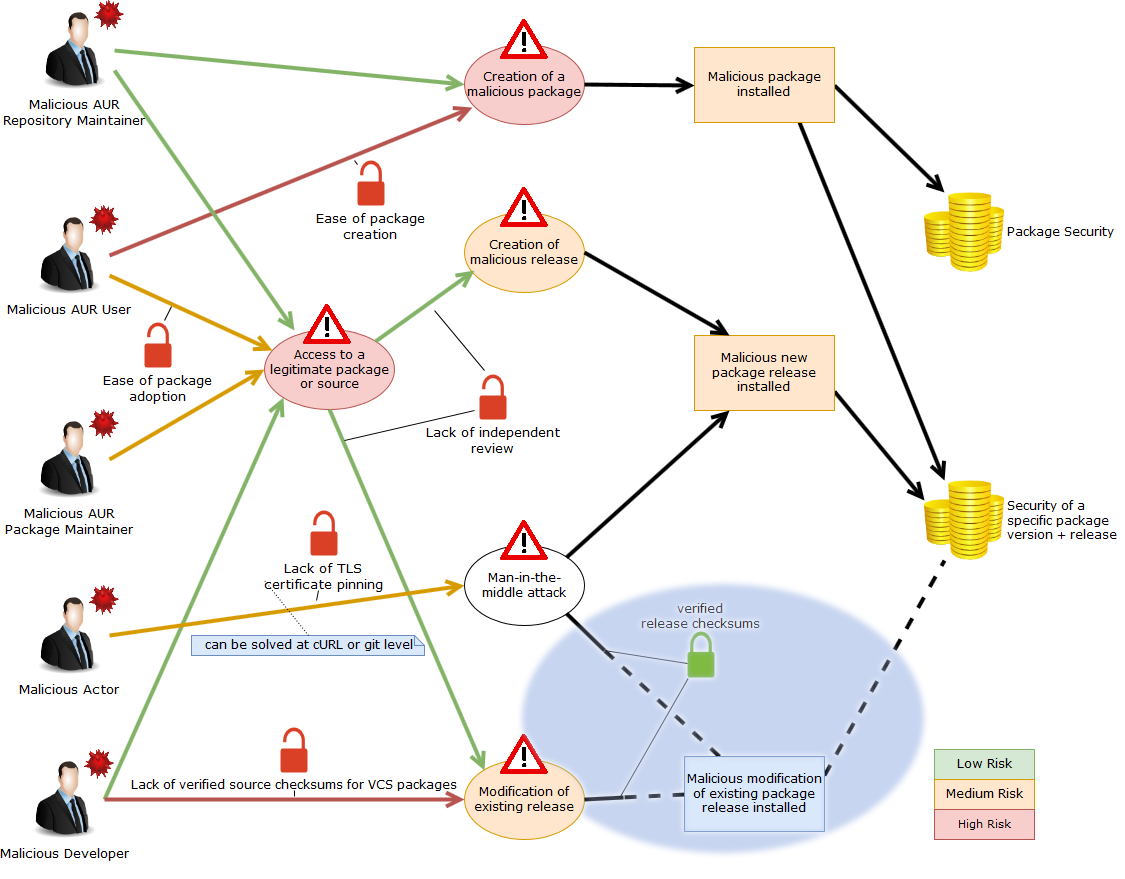
\includegraphics[width=\textwidth]{threat2n}
	\caption[Threat Prevention Strategy]{Strategy for Improving the Security of the AUR}
	\label{fig:threat2}
\end{figure}

Defence against the two attack scenarios mentioned in Section \ref{sec:attack_scenarios} requires the availability of cryptographically secure release hashes for every version of every package (Figure \ref{fig:threat2}).
If those were available, an attack would result in a hash mismatch and therefore the user could be warned.
However, the focus of the AURs design on simplicity, automation and fast package updates prevents any secure implementation on the server side as it would require the introduction of a central point of trust. That trust could only be maintained through the introduction of manual auditing, which is the opposite of what the AUR was designed for.

The solution must therefore be to implement a (preferably distributed) database on the user side, which means that there is no single authoritative source.
Since the aim is to defend against \emph{targeted} attacks, the assumption being that only comparatively few users will encounter a malicious version, this can be circumnavigated by checking the hash against a \emph{consensus} formed by many users.

% TODO: @important @lukas @bennett This paragraph is probably still unclear... need to think about that!
To make the database as safe as possible, a blockchain is used. The chain contains a smart contract providing securely callable functions. With one of these functions it is possible to commit a hash for a specific package and version.
This hash will be saved in the blockchain only if this user has not committed the same hash before, thereby making it harder to take over the blockchain and get a malicious hash to be the consensus.
The consensus is updated after every hash commit. Another function is used to get the current consensus hash and its valid commit count for a specific package and version.

This is the first project to use a blockchain as a means to provide distributed verification of (software) downloads.

% Workflow
\subsection{Workflow}
\label{sec:workflow}
The following workflow is visualized in Figure \ref{fig:main_workflow}.
\begin{figure}[!htb]
	\centering
		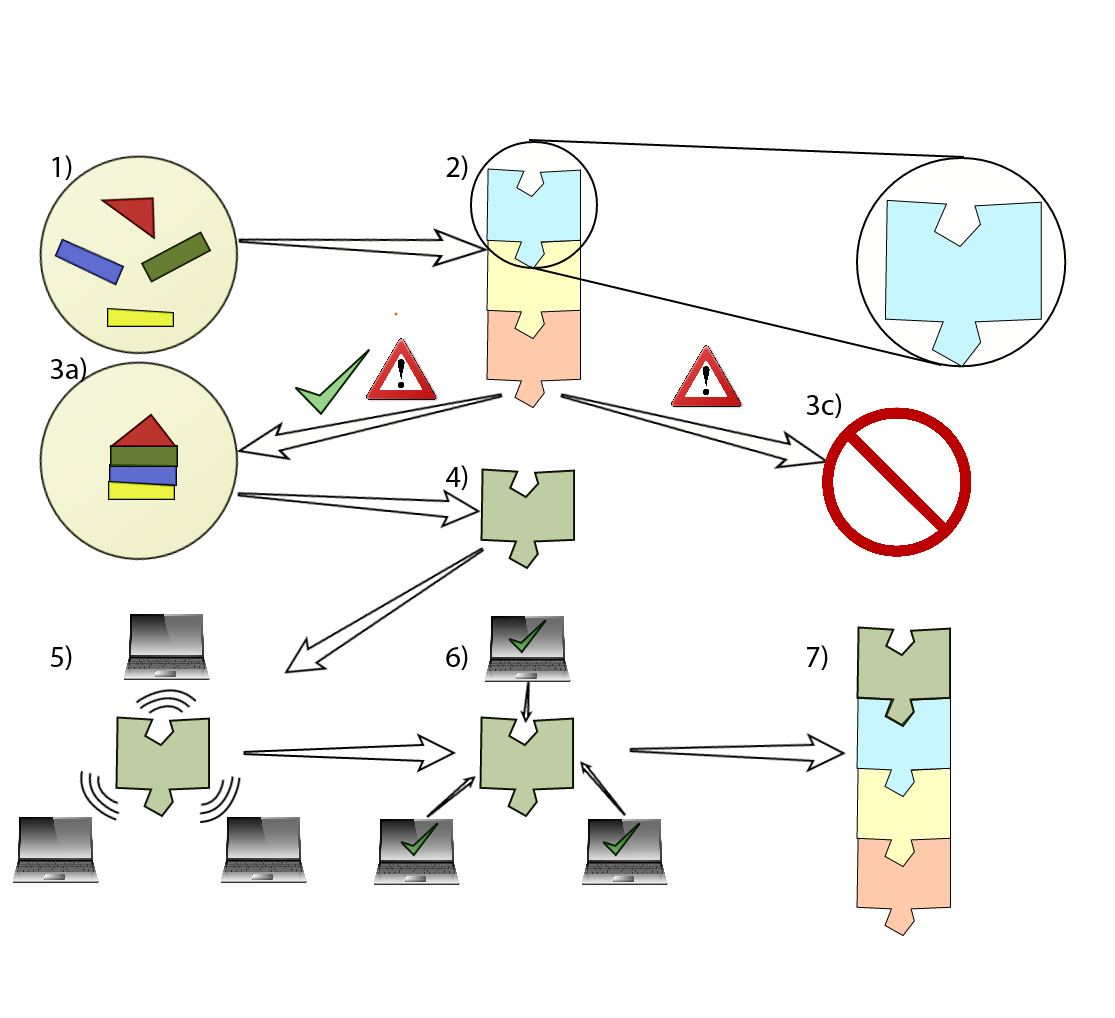
\includegraphics[width=0.6\paperwidth]{Workflow2}
	\caption{Main (Blockchain) Workflow}
	\label{fig:main_workflow}
\end{figure}

\begin{figure}[!htb]
	\centering
		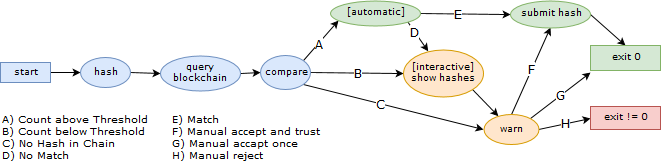
\includegraphics[width=\textwidth]{decision2}
	\caption{Aursec State Machine}
	\label{fig:state_machine}
\end{figure}


First of all a \texttt{PKGBUILD} is downloaded and partially executed in a sandbox in order to get the package version and download VCS sources (1).
Then, it is hashed along with any VCS sources and \texttt{.install} files.
The resulting local hash is compared with the current consensus (most often committed) hash of this package-version on the blockchain (2).

Depending on the comparison of the hashes (3), one of three things will happen [Figure~\ref{fig:state_machine}]:
The package may be created, installed and the hash will be added to the blockchain \emph{(Followed by step 4)} if the hashes match and the number of commits is above the trust threshold or the user decides to trust the locally generated hash anyway (A, F).

The package may be created and installed but the hash will not be added to the blockchain if the hashes do not match and/or the number is below the threshold, but the user wants to create and install the package without committing the hash. In this case the program exits with a zero status (B \rightarrow~G).

The package may not be created and installed because the hashes do not match and/or the number is below the threshold and the user doesn't want to create the package. In this case the program exits with a non-zero status (H).

If the locally generated hash is trusted, the local hash is committed to the blockchain (4). This is a transaction [see \texttt{aursec-chain commit-hash)}].
All nodes in the blockchain get the transaction over the network (5) and the transaction will be verified (together with all other transactions since the last block) and included the next mined block (6).
This mined block is then added to the blockchain (7).
As the transaction is included in a mined block, the consensus is atomically updated to reflect the new hash submission.
 %LUKAS
    \subsection{Blockchain implementation}\label{sec:aur-block}
In our approach we used Ethereum as blockchain and Solidity as the programming language for the smart contract.
We have chosen Ethereum because our blockchain has to fulfill several requirements:

Since we target Arch Linux, it must be easy to install on this platform.
This is covered by the \emph{geth} package which is available in the official community repository and can be directly installed using pacman.
The blockchain also needs to provide an API which allows external scripts to work with it.

Ethereum provides two APIs:
An IPC (interprocess communication) API, which allows connecting an interactive \emph{geth} console to a running blockchain, but is not convenient for external scripts,
and an HTTP RPC (remote procedure call) API which allows to send HTTP requests containing JSON bodies.
These requests can be sent with external scripts and programs since nearly every programming and scripting language (including bash) has HTTP support.
In our approach the shell script \texttt{aursec-chain}~(Section~\ref{sec:aursec-chain}) and the Python script \texttt{aursec-tui}~(Section~\ref{sec:tui}) use this API to interact with the blockchain.

The blockchain also needs to support smart contracts in order to allow us to use the blockchain functionally.
Ethereum not only supports smart contracts, they are it's main feature.
The specially developed high-level language \emph{Solidity} allows to write smart contracts in little time.

Our smart contract (Appendix~\ref{sec:contract}) provides two public functions which allow users to submit hashes (line 56) and to request the current consensus hash of a versioned package (line 43).
The contract allows each user to commit a hash only once: further commits of the same hash by the same user will not be considered in order to prevent manipulation of the consensus. This is implemented by keeping track of who submitted a hash (lines 58-60).

Finally, the blockchain needs to to provide an easy way to create private networks separate from the main one.
It would be safer to use the main blockchain because larger chains are harder to manipulate, and miners would get currency worth real money (in addition to secure software downloads) for their work, but we decided against that because the main blockchain takes up a lot of disk space and has much higher mining costs than makes sense for our application.
Ethereum provides possibilities to create private networks easily; It is only required to choose a network ID and to host the bootnode that is required to build the peer to peer network.
Our bootnode is active 24/7 on a DigitalOcean droplet provided by our supervisor.
Appendix \ref{sec:init-boot} explains how a new bootnode is added to the aursec-network.
 % LUKAS
    \subsection{Initialization - aursec-init}\label{sec:aursec-init}
Aursec-init is a shell script which allows the user to create all requirements for using our project.
It can also be used to rebuild the local copy of the blockchain, effectively re-installing from scratch.

First, it creates all needed folders and markers.
These markers track when hash commits and mining take place and are used by the systemd-service \textit{aursec-blockchain-mine} to adjust the mining effort based on recent hash commits.
Then, it creates the blockchain from our \emph{genesis block}, which is the first block in the blockchain.
After that, the synchronization of the blockchain begins.
In the meantime, the generation of the first two \emph{Directed Acyclic Graphs} (DAG) is stated.
Every DAG is a \~1GB dataset which is needed for mining new blocks \cite{wiki:DAG}.
Finally, the script mines a few blocks to gain enough currency to enable committing of hashes right after the initialization.
 % LUKAS
    \documentclass[11pt]{scrartcl}

%\usepackage[utf8]{inputenc} % use UTF-8 as input encoding - not necessary with xelatex
%\renewcommand{\baselinestretch}{2} % Line height
\usepackage[T1]{fontenc} % make non-ASCII characters cut&pastable in PDF
\usepackage{lmodern} % easiest way to get outline fonts with T1 encoding
\usepackage[english=american]{csquotes} % automatic quotation style
\usepackage[american]{babel}
\usepackage{abstract}

\usepackage{amsmath,amssymb} % math
\usepackage{caption} % For caption*
\usepackage[hidelinks, colorlinks=true]{hyperref} % Make links from things

\usepackage{graphicx} % images
\DeclareGraphicsExtensions{.eps,.pdf,.png,.jpg,.gif}
\graphicspath{{./img/}}
\usepackage{tabularx} % tabulars
\usepackage{array,booktabs} % rules for frontpage
\usepackage{titling} % "vars" for titlepage
\usepackage{minted} % syntax highlighting
\usepackage{csquotes} % display quotes
\usepackage{cleveref}
\usepackage{framed}
\usepackage{array}
\newcolumntype{L}[1]{>{\raggedright\let\newline\\\arraybackslash\hspace{0pt}}m{#1}}
\newcolumntype{C}[1]{>{\centering\let\newline\\\arraybackslash\hspace{0pt}}m{#1}}
\newcolumntype{R}[1]{>{\raggedleft\let\newline\\\arraybackslash\hspace{0pt}}m{#1}}


% Setup the page geometry
\usepackage[a4paper,top=3cm,bottom=3cm,left=3cm,right=3cm]{geometry}
%\usepackage[a4paper,margin=5cm,top=3cm,bottom=3cm,left=2.7cm,right=2.7cm]{geometry}



\title{AURsec}
\newcommand{\titlesub}{Detecting and preventing targeted attacks in the Arch User Repository: A~blockchain-based~approach}
\author{Bennett Piater \& Lukas Krismer}
\newcommand{\leader}{Supervisor: Christian Sillaber}
\newcommand{\university}{University of Innsbruck}
\newcommand{\course}{Bachelor thesis}
\date{\today}

\begin{document}
  %%% Boilerplate
  \thispagestyle{empty}

  %frontpage
  \input{frontpage.tex}

  % \input{formal}f


  \pagenumbering{Roman}
  \begin{abstract}
    \input{abstract}
  \end{abstract}

  \section*{Foreword}
  \input{foreword.tex}
  \pagebreak


  \tableofcontents
  \listoffigures
  % \listoftables
  \pagebreak


  %%% Content starts here
  \pagenumbering{arabic}

  \section{Introduction}  %(1/2 page)
    \input{intro}

  \section{Related Work}
    \input{background}
    \input{otherApproaches}

  \section{Motivation: Security Issues of the AUR} %(1 1/2 pages)
    \label{sec:security_issues}
    \input{security_issues} % BENNETT

  \section{AURsec}
    % TODO: maybe main tool - aursec; initialization - aursec-init; API - aursec-chain
    \input{core_solution} %LUKAS
    \input{detailedDescription/blockchain} % LUKAS
    \input{detailedDescription/aursec-init} % LUKAS
    \input{detailedDescription/aursec} % Bennett
    \input{detailedDescription/aursec-chain} % LUKAS
    \input{detailedDescription/systemd} % Bennett
    \subsection{Terminal User Interface} %(1/2 page)
    \input{tui}
    \subsection{Integration with AUR Helpers} \label{sec:integration}
    In order to achieve a meaningful security improvement for most users, integrations with common AUR helpers are necessary because hardly anyone builds AUR packages by hand.

    We focused on \texttt{aurutils}~\cite{gh:aurutils} because it is one of the few AUR helpers focused on security, which is also the reason why we use it in our daily life.

    After some discussion with its author, Alad Wenter, we decided to provide a wrapper which integrates \texttt{aursec} with \texttt{aurutils}; It's existing users can now take advantage of our improved security with minimal effort.

  % NOTE: Maybe in the appendix
  %\section{Lessons learned} %(1 page)
    %\input{learned.tex}
  \section{Evaluation}
    \input{eval}

  \section{Discussion}
    \input{discussion}

  % TODO: conclusion:

  \appendix
  \include{appendix}


  %%% Content ends here
  \pagebreak
  \bibliographystyle{plain}
  \bibliography{Literature.bib}

\end{document}
 % Bennett
    \subsubsection{API - aursec-chain}\label{sec:aursec-chain}
\texttt{aursec-chain} is a shell script which allows the user and other scripts to interact with our blockchain.
The script itself communicates with the blockchain through the JSON RPC.
It provides the commands to start and stop mining, mine a number of blocks, get the current consensus hash of a versioned package and commit a hash of a versioned package.
In our command pipeline, \texttt{aursec-verify-hashes} calls \texttt{aursec-chain get-hash \$ID}.
For our example \texttt{PKGBUILD}, the command looks like this:

\begin{verbatim}
aursec-chain get-hash aursec-git-v0.11.r0.15ea0e9-1
\end{verbatim}

this returns

\begin{verbatim}
c54d99fb6c4797cd994fcef74082396aaadbbcf44021932e04c65b77745e45cd 2
\end{verbatim}

which means that \texttt{\ldots745e45cd} is the current consensus hash and it was committed two times.

Furthermore \texttt{aursec} calls \texttt{aursec-chain commit-hash \$ID \$HASH} when the local hash is trusted in order to include it in the blockchain and update the consensus.

For our example \texttt{PKGBUILD}, the command looks like this:

\begin{verbatim}
aursec-chain commit-hash aursec-git-v0.11.r0.15ea0e9-1
		0bccd006ecf636e91cc924a7e6f9f25c26164de715c8972d146505b8e7ec1afc
\end{verbatim}

\texttt{aursec-chain} is also indirectly used by the systemd-service \texttt{aursec-blockchain-mine.timer}, which periodically mines blocks.
 % LUKAS
    \subsection{Systemd Services} \label{sec:aursec-systemd}
Since Arch Linux uses Systemd as init system and service manager, it was natural for this project to use it as well.

We use it for two things:

\paragraph*{aursec-blockchain.service} This service simply starts the blockchain process with the correct arguments. Using Systemd gives us an easy way to start the blockchain on boot with the correct configuration and a CPU quota to limit the impact on other running programs.

\paragraph*{aursec-blockchain-mine.timer} This timer is used to periodically mine blocks on the chain, thereby making the next wave of hashes available to other users. A Systemd timer works similarly to a Cron job, but with more control, and is easier to provide in a package.
 % Bennett
    \subsection{Terminal User Interface} %(1/2 page)
    \label{sec:tui}
\texttt{aursec-tui} is a urwid-based Python script. The TUI gives an overview over all mined blocks, their hashes, the miner of the block and any transactions which are saved in the block.

It is split in two parts. The first part is needed to gain the data from the blockchain and save it, the other part formats the information and displays it.
To display the results as fast as possible, the data is fetched in a background thread.
Any additional data will be displayed after the next refresh.
The script offers the user two settings for filtering the results:
\emph{only mine} shows all blocks which were mined by the user himself,
while \emph{only transactions} shows all blocks which contains at least one transaction.
The settings can be combined with the result that all blocks mined by the user and containing transactions will be displayed.
All hash-commit transactions are parsed into readable text.
Any other transaction is shown with the text \emph{``Transaction is no hash-commit''}.

    \subsection{Integration with AUR Helpers} \label{sec:integration}
    In order to achieve a meaningful security improvement for most users, integrations with common AUR helpers are necessary because hardly anyone builds AUR packages by hand.

    We focused on \texttt{aurutils}~\cite{gh:aurutils} because it is one of the few AUR helpers focused on security, which is also the reason why we use it in our daily life.

    After some discussion with its author, Alad Wenter, we decided to provide a wrapper which integrates \texttt{aursec} with \texttt{aurutils}; It's existing users can now take advantage of our improved security with minimal effort.

  % NOTE: Maybe in the appendix
  %\section{Lessons learned} %(1 page)
    %% Ethereum - Solidity
% RPC
% Bash as a programming language
% Python - Urwid

\subsubsection*{Ethereum --- Solidity}
Programming on a blockchain is a very interesting concept, but it seemed like it would take some getting used to. Thankfully, Solidity, the main language used on Ethereum, is a cleanly designed language which abstracts the blockchain away very nicely.

In practice, writing for Ethereum turned out to be enjoyable. Solidity reads like a half-way mix between C and Javascript, and most things that we rely on in this project happen automatically: Guaranteeing that the code cannot be modified, the ACID properties of transactions, etc. Solidity even supports some automatic formal verification, but not yet for \texttt{struct}s, so we cannot make use of it for our program.

All in all, Solidity is ideally suited for writing secure, \enquote{intelligent} (self-enforcing) databases.

\subsubsection*{JSON RPC}
The JSON PRC is used by \texttt{aursec-chain} for remote access to the block. Methods can be called or transactions can be sent by sending a JSON Object to the block chain. The answer from the block chain is also always a JSON Object. We learned how to parse JSON using python- and bash scripts. The best example is visible in the code of aursec-tui (Section~\ref{sec:tui}).

\subsubsection*{Bash}
Using Bash as a programming language was interesting. The language has many pitfalls~\cite{bash:pitfalls} and its syntax can be strange, even arcane; At the same time, we were often surprised by the advanced features that are provided directly by the language, such as string substitutions, regular expression matching or associative arrays.

These are the lessons that we learned about Bash (and whish we had known from the start):

\begin{itemize}
	\item Treat it as a functional programming language while structuring a program --- design in pipelines/streams.
	\item Error handling is hard to do well.
	Whenever possible, use \texttt{set -e} to abort on error and exit handlers for cleanup.
	\item Use a static analysis tool such as \emph{Shellcheck}~\cite{bash:shellcheck} to navigate the syntactic pitfalls.
	\item Find or invent a good way to test.
\end{itemize}

Bash doesn't provide or recommend a canonical testing framework, but associative arrays and \texttt{eval} allowed us to write our own system for basic unit tests with named test cases, commands to execute, and expected invariants.
We used it to great effect in narrowing down the best \texttt{firejail} sandbox ruleset, e.g. preventing \texttt{makepkg} from writing to folders other than \texttt{pwd}.

Overall, Bash is powerful and probably the perfect tool for this job, but so different from common programming languages that it took some getting used to.

\subsubsection*{Python-Urwid}
Urwid \cite{urwid} is a \emph{Terminal User Interface} (TUI) library for Python. It provides ready-made widgets which make it easy to create structured user interfaces. In total there are 20 different Widget-Classes which differ in type (box/flow/fixed) and category (basic/graphic/decoration/container). The basic and the graphic widgets contain the content. The decoration and container widgets are used to structure the TUI.

Buttons, check-boxes and key bindings allow to call functions. This function may add, remove or change widgets on runtime.

Using this library, we learned how to write simple TUIs which are completely modular and can be extended anytime.

  \section{Evaluation}
    % AUR:
% SHOW THE 2 ATTACK EXAMPLES MENTIONED ABOVE
% (MALICIOUS MAINTAINER AND VCS ATTACK USING SHA1 COLLISION)

% - Bauerbill (detects maintainer changes; allows trusting maintainers globally, for specific packages, or for specific package-timestamp combinations)
% - Aurutils (aursync allows verifying all downloaded build files at once before proceeding with the source download and installation)
\label{sec:eval}
\subsection{Effectiveness of AURsec}\label{sec:security_comparison}
Two notable AUR helpers provide some degree of security: \texttt{aurutils}~\cite{gh:aurutils}, which at least incentivizes users to inspect build files before installing a package, and \texttt{bauerbill}~\cite{bauerbill}, which also provides a local trust management system.
The most common AUR helper, \texttt{yaourt}, disincentivizes users from checking build files because it takes multiple manual steps for each package to do so.

In order to evaluate the performance of \texttt{aursec}, we compared how well it fared against the other two tools in the two attack scenarios that we identified in Section~\ref{sec:attack_scenarios}.

In the scenario from Section~\ref{sec:maint_attack}, the assumption is that a malicious maintainer conducts a targeted attack against an AUR user by temporarily modifying the build files.
\texttt{aurutils} allows users to manually verify build files in bulk using a VIM-style file manager before proceeding, and also shows diffs from the previous version if that is available.
Security-conscious and attentive users may therefore catch the malicious modification --- but only if it is not innocuous enough.
For example, an attacker could change the upstream URL to one that looks equally legitimate (but containing malicious code) and adapt the checksums appropriately, in which case most users wouldn't stand a chance.
In addition to manual verification, \texttt{bauerbill}s trust management system would warn the user if the maintainer of the package changed (such as during adoption of an orphan package), an example of which can be seen in Figure~\ref{fig:bb-query_trust}.
However, if the attack doesn't rely on taking over an orphan package because the existing maintainer is malicious, his SSH key was compromised, or similar, \texttt{bauerbill} doesn't provide more security than \texttt{aurutils}.
\texttt{aursec} easily detects this attack (as long as enough users participate for a useful consensus to have been formed) because the malicious modification would trigger a hash mismatch, of which the user would be warned as seen in Section~\ref{sec:aursec}

\begin{figure}
	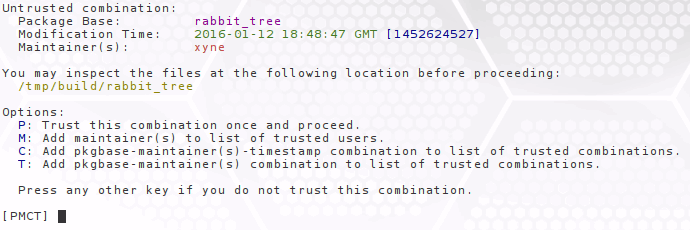
\includegraphics[width=\linewidth]{img/bb-query_trust-screenshot.png}
	\caption{Bauerbills trust management system \cite{bauerbill}}
	\label{fig:bb-query_trust}
\end{figure}

In the scenario from Section~\ref{sec:vcs_attack}, the assumption is that an upstreams VCS repository was attacked or made malicious changes.
No AUR helper is capable of detecting this attack because source integrity verification is normally handled my \texttt{makepkg}. If no checksums are available in the PKGBUILD, such as is the case for VCS packages, nothing can be done with the existing infrastructure.
However, \texttt{aursec} handles this exactly like it handles the previous attack because it hashes VCS sources in addition to the build files.

Therefore, \texttt{aursec} provides superior protection to existing solutions. The comparison is summarized in Table~\ref{tab:defence-comparison}.

\begin{table}
	\centering
	\begin{tabular}{l|m{3cm}|c|m{3cm}}
	\hline

	\hline
	\textbf{Detected Attack} & \textbf{AURsec} & \textbf{Bauerbill} & \textbf{aurutils} \\
	\hline
		Maintainer change & any change without new version & yes & no \\
		Modified build files & yes & manually & manually, diffs between versions \\
		Manipulated VCS sources & yes & no & no \\
	\hline

	\hline
	\end{tabular}
	\caption{Comparison of defence methods against our attack scenarios}
	\label{tab:defence-comparison}
\end{table}

% OTHER PACKAGE MANAGERS:
% EXPLAIN THAT THEY ARE INSECURE AS S**T
% AND THAT OUR APPROACH COULD BE ADAPTED TO THEM,
% allthough not as easily because the AUR has modular helpers already,
% whereas adapting to the other platforms would require forking/patching more monolithic tools or building custom ones

\subsection{Applicability to other packaging systems} % TODO: @lukas better wording instead of "community packaging systems"?
As noted in the introduction, other community packaging systems share security issues with the AUR, which means that most of the analysis from Section~\ref{sec:security_issues} also applies to them.
The \emph{Python Package Index} allows signing of packages with GPG, but its client (\texttt{pip}) cannot verify them~\cite{pypi:security}, so users would need to do that by hand.
There is also no web of trust or any similar mechanism, so users would need to build trust in every individual maintainer.
This is exactly the same situation as that of the AUR.

The \emph{Node package manager} is even worse: There is no means for any signing whatsoever~\cite{npm:security}.

Out of all community package managing systems we looked at, \emph{rubygems.org} is the only one that is open about the state of its security, but they also have the same problems:

\begin{displayquote}
RubyGems has had the ability to cryptographically sign gems since version 0.8.11. This signing works by using the gem cert command to create a key pair, and then packaging signing data inside the gem itself. The gem install command optionally lets you set a security policy, and you can verify the signing key for a gem before you install it.

However, this method of securing gems is not widely used. It requires a number of manual steps on the part of the developer, and there is no well-established chain of trust for gem signing keys. Discussion of new signing models such as X509 and OpenPGP is going on in the rubygems-trust wiki, the RubyGems-Developers list and in IRC.~\cite{rubygems:security}
\end{displayquote}

The communities of the above community packaging systems have been talking about security improvements for years (since about 2012 in most cases), but no significant work has been done to this day.
Since it works purely on the client side and doesn't require any modifications to infrastructure, the solution implemented by AURsec would also be applicable to these other systems.

However, it would take much more work than for the AUR because of the different nature of the ecosystems.
While the AUR is one central location, there is no official client for it, so many users use it by hand and a wide range of (often easily extensible) AUR helpers is available.
This makes it comparatively easy for people to use \texttt{aursec} with their existing workflow.
In contrast, the other community packaging systems each have \emph{one} monolithic official client, and none of them have sufficient hook or plugin mechanisms to make them extensible enough for something like AURsec, so adapting our work to those platforms would require creating custom clients or the distribution of patched versions of the official ones.


  \section{Discussion}
    \label{sec:discuss}
Simulated attacks of the kind discussed in Section \ref{sec:attack_scenarios} have been detected effectively in our experiments, and the core toolchain is convenient to use and performant.
Also synchronization between users and automatic mining works as expected.

However, our approach has several major disadvantages that necessarily follow from using a blockchain: Every user must have a full copy of the chain on his machine, which requires a non-negligible amount of hard drive memory at best.
The local copies must also be kept in sync, which requires a background process and near-permanent network connection.
Finally, the fact that we need a high mining difficulty to prevent the spreading of fake hashes makes our system very computationally expensive for what it is.

\subsection{Alternatives}
There are other conceivable ways of securing the AUR on the user side.
The most obvious one would be to do away with the blockchain and replace it with a traditional database accessible through a web service.

That approach has the advantage of being much lighter and more straightforward to use, as it doesn't need local blockchain copies, background processes or periodic mining on every client machine. However, it achieves that by creating a single point of failure (the web service) and a new trust requirement (in the owners of the web service).

In the end, the choice between these approaches involves a trade-off between computational costs and client-side complexity on the one hand, and basic trust on the other.

Other approaches would be the creation of a new, trusted source repository downstream of the AUR, requiring trust in a central authority, or a complete re-design of the AUR itself at the cost of ease of use. Neither of these is particularly appealing, allthough the former is very sensible for specific uses and/or closed organizations, and is already being used for those cases.


\subsection{Future Work}
The system would need several months of testing with hundreds of users in order to assess its actual performance, so we are looking forward to more engagement from the community when AURsec advances.
To date, we have not received enough feedback or run our project with enough people to draw meaningful conclusions.

However, we have already started working on a large update that will make the system more secure.
The main improvement is an extended smart contract that does not merely return the most common hash and its submission count, but also returns the count for the second most common hash.

This will allow us to factor the proportion between the two counts into the trust instead of the current simple trust threshold.
We also need to address the mining difficulty: that is, the system must be usable, but at the same time hard to manipulate. This will require more testing.
Depending on the mining difficulty that we choose, we might also make the periodic mining mine for a set time instead of a set number of blocks, in order to adjust the mining-effort of each user .
Finally, we want to use Systemd's cgroups resource management more effectively in order to limit the performance and battery impact of running our project in the background.


  % TODO: conclusion:

  \appendix
  \section{A sample \texttt{PKGBUILD}}\label{sec:our-pkgbuild}

\begin{minted}[linenos]{bash}
# Maintainer: Bennett Piater <bennett at piater dot name>

pkgname=(aursec-git aursec-tui-git)
pkgver=v0.11.r0.15ea0e9
pkgrel=1
pkgdesc='Verify AUR package sources against hashes stored in a blockchain.'
arch=(any)
url="https://github.com/clawoflight/${pkgbase%-git}"
license=('custom:MPL2')

provides=("${pkgname%-git}")
conflicts=("${pkgname%-git}")

depends=(firejail geth vim bc)
makedepends=(pandoc git)
checkdepends=(shellcheck)

source=("git+https://github.com/clawoflight/${pkgname%-git}.git")
sha256sums=('SKIP')
validpgpkeys=('871F10477DB3DDED5FC447B226C7E577EF967808')

pkgver() {
    cd "${pkgname%-git}"
    printf "%s" "$(git describe --long | sed 's/\([^-]*-\)g/r\1/;s/-/./g')"
}

build() {
    cd "${pkgname%-git}/aursec"
    make
    cd "../tui"
    make
}

check() {
    cd "${pkgname%-git}/aursec"
    make -k check
}

package_aursec-git() {
    install=aursec-git.install
    optdepends=("aursec-tui: to manually inspect the blockchain.")

    cd "${pkgname%-git}/aursec"
    make PREFIX="/usr" DESTDIR="$pkgdir/" install
}

package_aursec-tui-git() {
    pkgdesc='Inspect the aursec blockchain'
    depends=(python python-requests python-urwid aursec)
    provides=(aursec-tui)
    conflicts=(aursec-tui)

    cd "aursec/tui"
    make PREFIX="/usr" DESTDIR="$pkgdir/" install
}
\end{minted}

\section{Smart Contract}\label{sec:contract}
\begin{minted}[linenos]{javascript}
// This Source Code Form is subject to the terms of the Mozilla Public
// License, v. 2.0. If a copy of the MPL was not distributed with this
// file, You can obtain one at http://mozilla.org/MPL/2.0/.
// Copyright 2016-2017 Lukas Krismer and Bennett Piater.

pragma solidity ^0.4.0;
import "contracts/Owned.sol";

/**
 * @title Registry of AUR package hashes
 * @author Bennett Piater
 */
contract AURPackageRegistry is Owned {

    // Struct that holds the consensus
    // and the number of submissions for each hash for a package.
    struct PackageData {
        string currentConsensusPkgHash;
        mapping (string => uint) timesHashSubmitted;
    }

    // Map package IDs "$pkgname-$pkgver-$pkgrel" to the corresponding struct
    mapping (string => PackageData) packages;

    // Map a hash to a map of blockchain wallet addresses (users).
    // This allows checking whether a user submitted a hash.
    mapping (string => mapping (address => bool)) addressesThatSubmittedAHash;

    event PkgHashSubmitted(string indexed packageID, string pkgHash,
        uint submissionCount, address indexed submitter);
    event ConsensusFormed(string indexed packageID, string pkgHash,
        uint submissionCount);

    /**
     * @notice Get the current consensus and how many nodes submitted it
     * for a given package,version,release combination.
     *
     * @param packageID The id of the package to submit: pkgname-pkgver-pkgrel
     *
     * @return pkgHash The hash of the package, or the empty string if none is stored.
     * @return submissionCount The number of nodes that submitted this hash
     */
    function getCurrentConsensus(string packageID) constant
    returns (string pkgHash, uint submissionCount) {
        string hash = packages[packageID].currentConsensusPkgHash;
        return (hash, packages[packageID].timesHashSubmitted[hash]);
    }

    /**
     * @notice Submit a new hash for a package.
     *
     * @param packageID The id of the package to submit: pkgname-pkgver-pkgrel
     * @param pkgHash The hash of the package
     * @return success Whether the submission succeeded
     */
    function submitPkgHash(string packageID, string pkgHash) returns (bool success) {
        // Only allow every address (=user) to submit a hash once
        if (addressesThatSubmittedAHash[pkgHash][msg.sender])
            return false;
        addressesThatSubmittedAHash[pkgHash][msg.sender] = true;

        PackageData package = packages[packageID];
        package.timesHashSubmitted[pkgHash] += 1;
        // Trigger notification
        PkgHashSubmitted(packageID, pkgHash,
            package.timesHashSubmitted[pkgHash], msg.sender);

        // If this hash has become the new consensus
        if (package.timesHashSubmitted[pkgHash] >
            package.timesHashSubmitted[package.currentConsensusPkgHash]) {

            package.currentConsensusPkgHash = pkgHash;
            // Trigger notification
            ConsensusFormed(packageID, pkgHash, package.timesHashSubmitted[pkgHash]);
        }

        return true;
    }
}
\end{minted}

\newpage
\section{Adding Bootnodes}\label{sec:init-boot}
This section explains how mining and non-mining bootnodes can be created and integrated into our network.\newline

\textbf{Mining bootnodes} can only be initialized automatically with \emph{aursec-init} on Arch Linux.
After doing so, instead of starting the systemd services, use the command
\begin{verbatim}
sudo su aursec -c '/usr/bin/geth --fast --port 30200 --rpcport 8105 --nodiscover
--ipcdisable --rpc --rpcapi "eth,web3,miner" --datadir /var/aursec/chain --cache 512
--networkid 42 --verbosity 4 --unlock 0 --password /var/aursec/password console'
\end{verbatim}

to get a geth console. To get your node-url run \texttt{admin.nodeInfo}. Copy the url and close the console (Ctrl+D or exit). To start the node use

\begin{verbatim}
sudo su aursec -c '/usr/bin/geth --fast --port 30200 --rpcport 8105 --nodiscover
--ipcdisable --rpc --rpcapi "eth,web3,miner" --datadir /var/aursec/chain --cache 512
--networkid 42 --verbosity 4 --unlock 0 --password /var/aursec/password'
\end{verbatim}

Now start the \texttt{aursec-blockchain-mine.timer}.
To integrate the bootnode to the network, read the corresponding paragraph below.\linebreak

\textbf{Non-mining bootnodes} only require the \texttt{geth} package and can be set up on any system.
To initialize the bootnode run the following commands:
\begin{verbatim}
> bootnode -genkey $PathToKeyfile
> bootnode -nodekey $PathToKeyfile -addr 30200
\end{verbatim}
The node-url will be shown in the first line after the second command.
To integrate the bootnode into the network, read the following paragraph.


\paragraph*{Integrate the Bootnode}
Copy the node-url consisting of \texttt{nodeUrl@yourip:30200} to our \texttt{aursec-blockchain.service} \footnote{https://github.com/clawoflight/aursec/blob/master/aursec/lib/aursec-blockchain.service} after the \texttt{--bootnodes} argument and submit a pull request.


\newpage
\section{Contributions}\label{sec:resp}
We split our work into areas of responsibility for which one of us was responsible (see Table \ref{tab:responsibilities}). However, usually both of us worked on any given area.
\begin{table}[!htb]
\centering
\caption{Contributions}
\label{tab:responsibilities}
\begin{tabular}{|l|L{5.5cm}|L{5.5cm}|}
\hline
Name & Code &  Paper \\ \hline
Bennett Piater & Solidity (Smart Contracts), automatic mining, hashing of packages, main command pipeline , aurutils wrapper, AUR-Packages   &
Abstract,
Motivation (Complete Section \ref{sec:motivation}),
AURsec (Main tool up to and including architecture, Systemd services, Integration with AUR Helpers ) ( \Cref{sec:aursec,sec:aur-architecture,sec:aursec-systemd,sec:integration} including Appendix \ref{sec:our-pkgbuild}),
Solidity code (Appendix \ref{sec:contract}),
Evaluation (Complete Section \ref{sec:eval}),
Discussion (Complete Section \ref{sec:discuss})
\\ \hline
Lukas Krismer &  Initialization of the blockchain, Integration of the contract, bash-API for ethereum , Terminal-User-Interface, Initialization of the bootnode &
Forword,
Introduction (Complete Section \ref{sec:intro}),
Related Work (Complete Section \ref{sec:related}),
AURsec(workflow, blockchain implementation, initialization, API, Terminal User Interface, bootnode) ( \Cref{sec:AURsec,sec:workflow,sec:aur-block,sec:aursec-init,sec:aursec-chain,sec:tui} including Appendix \ref{sec:init-boot}),
Contributions (Appendix \ref{sec:resp})\\ \hline
\end{tabular}
\end{table}




  %%% Content ends here
  \pagebreak
  \bibliographystyle{plain}
  \bibliography{Literature.bib}

\end{document}
 % Bennett
    \subsubsection{API - aursec-chain}\label{sec:aursec-chain}
\texttt{aursec-chain} is a shell script which allows the user and other scripts to interact with our blockchain.
The script itself communicates with the blockchain through the JSON RPC.
It provides the commands to start and stop mining, mine a number of blocks, get the current consensus hash of a versioned package and commit a hash of a versioned package.
In our command pipeline, \texttt{aursec-verify-hashes} calls \texttt{aursec-chain get-hash \$ID}.
For our example \texttt{PKGBUILD}, the command looks like this:

\begin{verbatim}
aursec-chain get-hash aursec-git-v0.11.r0.15ea0e9-1
\end{verbatim}

this returns

\begin{verbatim}
c54d99fb6c4797cd994fcef74082396aaadbbcf44021932e04c65b77745e45cd 2
\end{verbatim}

which means that \texttt{\ldots745e45cd} is the current consensus hash and it was committed two times.

Furthermore \texttt{aursec} calls \texttt{aursec-chain commit-hash \$ID \$HASH} when the local hash is trusted in order to include it in the blockchain and update the consensus.

For our example \texttt{PKGBUILD}, the command looks like this:

\begin{verbatim}
aursec-chain commit-hash aursec-git-v0.11.r0.15ea0e9-1
		0bccd006ecf636e91cc924a7e6f9f25c26164de715c8972d146505b8e7ec1afc
\end{verbatim}

\texttt{aursec-chain} is also indirectly used by the systemd-service \texttt{aursec-blockchain-mine.timer}, which periodically mines blocks.
 % LUKAS
    \subsection{Systemd Services} \label{sec:aursec-systemd}
Since Arch Linux uses Systemd as init system and service manager, it was natural for this project to use it as well.

We use it for two things:

\paragraph*{aursec-blockchain.service} This service simply starts the blockchain process with the correct arguments. Using Systemd gives us an easy way to start the blockchain on boot with the correct configuration and a CPU quota to limit the impact on other running programs.

\paragraph*{aursec-blockchain-mine.timer} This timer is used to periodically mine blocks on the chain, thereby making the next wave of hashes available to other users. A Systemd timer works similarly to a Cron job, but with more control, and is easier to provide in a package.
 % Bennett
    \subsection{Terminal User Interface} %(1/2 page)
    \label{sec:tui}
\texttt{aursec-tui} is a urwid-based Python script. The TUI gives an overview over all mined blocks, their hashes, the miner of the block and any transactions which are saved in the block.

It is split in two parts. The first part is needed to gain the data from the blockchain and save it, the other part formats the information and displays it.
To display the results as fast as possible, the data is fetched in a background thread.
Any additional data will be displayed after the next refresh.
The script offers the user two settings for filtering the results:
\emph{only mine} shows all blocks which were mined by the user himself,
while \emph{only transactions} shows all blocks which contains at least one transaction.
The settings can be combined with the result that all blocks mined by the user and containing transactions will be displayed.
All hash-commit transactions are parsed into readable text.
Any other transaction is shown with the text \emph{``Transaction is no hash-commit''}.

    \subsection{Integration with AUR Helpers} \label{sec:integration}
    In order to achieve a meaningful security improvement for most users, integrations with common AUR helpers are necessary because hardly anyone builds AUR packages by hand.

    We focused on \texttt{aurutils}~\cite{gh:aurutils} because it is one of the few AUR helpers focused on security, which is also the reason why we use it in our daily life.

    After some discussion with its author, Alad Wenter, we decided to provide a wrapper which integrates \texttt{aursec} with \texttt{aurutils}; It's existing users can now take advantage of our improved security with minimal effort.

  % NOTE: Maybe in the appendix
  %\section{Lessons learned} %(1 page)
    %% Ethereum - Solidity
% RPC
% Bash as a programming language
% Python - Urwid

\subsubsection*{Ethereum --- Solidity}
Programming on a blockchain is a very interesting concept, but it seemed like it would take some getting used to. Thankfully, Solidity, the main language used on Ethereum, is a cleanly designed language which abstracts the blockchain away very nicely.

In practice, writing for Ethereum turned out to be enjoyable. Solidity reads like a half-way mix between C and Javascript, and most things that we rely on in this project happen automatically: Guaranteeing that the code cannot be modified, the ACID properties of transactions, etc. Solidity even supports some automatic formal verification, but not yet for \texttt{struct}s, so we cannot make use of it for our program.

All in all, Solidity is ideally suited for writing secure, \enquote{intelligent} (self-enforcing) databases.

\subsubsection*{JSON RPC}
The JSON PRC is used by \texttt{aursec-chain} for remote access to the block. Methods can be called or transactions can be sent by sending a JSON Object to the block chain. The answer from the block chain is also always a JSON Object. We learned how to parse JSON using python- and bash scripts. The best example is visible in the code of aursec-tui (Section~\ref{sec:tui}).

\subsubsection*{Bash}
Using Bash as a programming language was interesting. The language has many pitfalls~\cite{bash:pitfalls} and its syntax can be strange, even arcane; At the same time, we were often surprised by the advanced features that are provided directly by the language, such as string substitutions, regular expression matching or associative arrays.

These are the lessons that we learned about Bash (and whish we had known from the start):

\begin{itemize}
	\item Treat it as a functional programming language while structuring a program --- design in pipelines/streams.
	\item Error handling is hard to do well.
	Whenever possible, use \texttt{set -e} to abort on error and exit handlers for cleanup.
	\item Use a static analysis tool such as \emph{Shellcheck}~\cite{bash:shellcheck} to navigate the syntactic pitfalls.
	\item Find or invent a good way to test.
\end{itemize}

Bash doesn't provide or recommend a canonical testing framework, but associative arrays and \texttt{eval} allowed us to write our own system for basic unit tests with named test cases, commands to execute, and expected invariants.
We used it to great effect in narrowing down the best \texttt{firejail} sandbox ruleset, e.g. preventing \texttt{makepkg} from writing to folders other than \texttt{pwd}.

Overall, Bash is powerful and probably the perfect tool for this job, but so different from common programming languages that it took some getting used to.

\subsubsection*{Python-Urwid}
Urwid \cite{urwid} is a \emph{Terminal User Interface} (TUI) library for Python. It provides ready-made widgets which make it easy to create structured user interfaces. In total there are 20 different Widget-Classes which differ in type (box/flow/fixed) and category (basic/graphic/decoration/container). The basic and the graphic widgets contain the content. The decoration and container widgets are used to structure the TUI.

Buttons, check-boxes and key bindings allow to call functions. This function may add, remove or change widgets on runtime.

Using this library, we learned how to write simple TUIs which are completely modular and can be extended anytime.

  \section{Evaluation}
    % AUR:
% SHOW THE 2 ATTACK EXAMPLES MENTIONED ABOVE
% (MALICIOUS MAINTAINER AND VCS ATTACK USING SHA1 COLLISION)

% - Bauerbill (detects maintainer changes; allows trusting maintainers globally, for specific packages, or for specific package-timestamp combinations)
% - Aurutils (aursync allows verifying all downloaded build files at once before proceeding with the source download and installation)
\label{sec:eval}
\subsection{Effectiveness of AURsec}\label{sec:security_comparison}
Two notable AUR helpers provide some degree of security: \texttt{aurutils}~\cite{gh:aurutils}, which at least incentivizes users to inspect build files before installing a package, and \texttt{bauerbill}~\cite{bauerbill}, which also provides a local trust management system.
The most common AUR helper, \texttt{yaourt}, disincentivizes users from checking build files because it takes multiple manual steps for each package to do so.

In order to evaluate the performance of \texttt{aursec}, we compared how well it fared against the other two tools in the two attack scenarios that we identified in Section~\ref{sec:attack_scenarios}.

In the scenario from Section~\ref{sec:maint_attack}, the assumption is that a malicious maintainer conducts a targeted attack against an AUR user by temporarily modifying the build files.
\texttt{aurutils} allows users to manually verify build files in bulk using a VIM-style file manager before proceeding, and also shows diffs from the previous version if that is available.
Security-conscious and attentive users may therefore catch the malicious modification --- but only if it is not innocuous enough.
For example, an attacker could change the upstream URL to one that looks equally legitimate (but containing malicious code) and adapt the checksums appropriately, in which case most users wouldn't stand a chance.
In addition to manual verification, \texttt{bauerbill}s trust management system would warn the user if the maintainer of the package changed (such as during adoption of an orphan package), an example of which can be seen in Figure~\ref{fig:bb-query_trust}.
However, if the attack doesn't rely on taking over an orphan package because the existing maintainer is malicious, his SSH key was compromised, or similar, \texttt{bauerbill} doesn't provide more security than \texttt{aurutils}.
\texttt{aursec} easily detects this attack (as long as enough users participate for a useful consensus to have been formed) because the malicious modification would trigger a hash mismatch, of which the user would be warned as seen in Section~\ref{sec:aursec}

\begin{figure}
	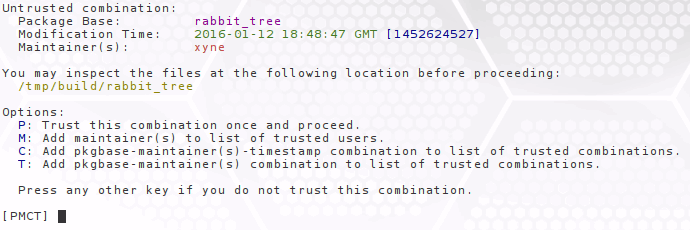
\includegraphics[width=\linewidth]{img/bb-query_trust-screenshot.png}
	\caption{Bauerbills trust management system \cite{bauerbill}}
	\label{fig:bb-query_trust}
\end{figure}

In the scenario from Section~\ref{sec:vcs_attack}, the assumption is that an upstreams VCS repository was attacked or made malicious changes.
No AUR helper is capable of detecting this attack because source integrity verification is normally handled my \texttt{makepkg}. If no checksums are available in the PKGBUILD, such as is the case for VCS packages, nothing can be done with the existing infrastructure.
However, \texttt{aursec} handles this exactly like it handles the previous attack because it hashes VCS sources in addition to the build files.

Therefore, \texttt{aursec} provides superior protection to existing solutions. The comparison is summarized in Table~\ref{tab:defence-comparison}.

\begin{table}
	\centering
	\begin{tabular}{l|m{3cm}|c|m{3cm}}
	\hline

	\hline
	\textbf{Detected Attack} & \textbf{AURsec} & \textbf{Bauerbill} & \textbf{aurutils} \\
	\hline
		Maintainer change & any change without new version & yes & no \\
		Modified build files & yes & manually & manually, diffs between versions \\
		Manipulated VCS sources & yes & no & no \\
	\hline

	\hline
	\end{tabular}
	\caption{Comparison of defence methods against our attack scenarios}
	\label{tab:defence-comparison}
\end{table}

% OTHER PACKAGE MANAGERS:
% EXPLAIN THAT THEY ARE INSECURE AS S**T
% AND THAT OUR APPROACH COULD BE ADAPTED TO THEM,
% allthough not as easily because the AUR has modular helpers already,
% whereas adapting to the other platforms would require forking/patching more monolithic tools or building custom ones

\subsection{Applicability to other packaging systems} % TODO: @lukas better wording instead of "community packaging systems"?
As noted in the introduction, other community packaging systems share security issues with the AUR, which means that most of the analysis from Section~\ref{sec:security_issues} also applies to them.
The \emph{Python Package Index} allows signing of packages with GPG, but its client (\texttt{pip}) cannot verify them~\cite{pypi:security}, so users would need to do that by hand.
There is also no web of trust or any similar mechanism, so users would need to build trust in every individual maintainer.
This is exactly the same situation as that of the AUR.

The \emph{Node package manager} is even worse: There is no means for any signing whatsoever~\cite{npm:security}.

Out of all community package managing systems we looked at, \emph{rubygems.org} is the only one that is open about the state of its security, but they also have the same problems:

\begin{displayquote}
RubyGems has had the ability to cryptographically sign gems since version 0.8.11. This signing works by using the gem cert command to create a key pair, and then packaging signing data inside the gem itself. The gem install command optionally lets you set a security policy, and you can verify the signing key for a gem before you install it.

However, this method of securing gems is not widely used. It requires a number of manual steps on the part of the developer, and there is no well-established chain of trust for gem signing keys. Discussion of new signing models such as X509 and OpenPGP is going on in the rubygems-trust wiki, the RubyGems-Developers list and in IRC.~\cite{rubygems:security}
\end{displayquote}

The communities of the above community packaging systems have been talking about security improvements for years (since about 2012 in most cases), but no significant work has been done to this day.
Since it works purely on the client side and doesn't require any modifications to infrastructure, the solution implemented by AURsec would also be applicable to these other systems.

However, it would take much more work than for the AUR because of the different nature of the ecosystems.
While the AUR is one central location, there is no official client for it, so many users use it by hand and a wide range of (often easily extensible) AUR helpers is available.
This makes it comparatively easy for people to use \texttt{aursec} with their existing workflow.
In contrast, the other community packaging systems each have \emph{one} monolithic official client, and none of them have sufficient hook or plugin mechanisms to make them extensible enough for something like AURsec, so adapting our work to those platforms would require creating custom clients or the distribution of patched versions of the official ones.


  \section{Discussion}
    \label{sec:discuss}
Simulated attacks of the kind discussed in Section \ref{sec:attack_scenarios} have been detected effectively in our experiments, and the core toolchain is convenient to use and performant.
Also synchronization between users and automatic mining works as expected.

However, our approach has several major disadvantages that necessarily follow from using a blockchain: Every user must have a full copy of the chain on his machine, which requires a non-negligible amount of hard drive memory at best.
The local copies must also be kept in sync, which requires a background process and near-permanent network connection.
Finally, the fact that we need a high mining difficulty to prevent the spreading of fake hashes makes our system very computationally expensive for what it is.

\subsection{Alternatives}
There are other conceivable ways of securing the AUR on the user side.
The most obvious one would be to do away with the blockchain and replace it with a traditional database accessible through a web service.

That approach has the advantage of being much lighter and more straightforward to use, as it doesn't need local blockchain copies, background processes or periodic mining on every client machine. However, it achieves that by creating a single point of failure (the web service) and a new trust requirement (in the owners of the web service).

In the end, the choice between these approaches involves a trade-off between computational costs and client-side complexity on the one hand, and basic trust on the other.

Other approaches would be the creation of a new, trusted source repository downstream of the AUR, requiring trust in a central authority, or a complete re-design of the AUR itself at the cost of ease of use. Neither of these is particularly appealing, allthough the former is very sensible for specific uses and/or closed organizations, and is already being used for those cases.


\subsection{Future Work}
The system would need several months of testing with hundreds of users in order to assess its actual performance, so we are looking forward to more engagement from the community when AURsec advances.
To date, we have not received enough feedback or run our project with enough people to draw meaningful conclusions.

However, we have already started working on a large update that will make the system more secure.
The main improvement is an extended smart contract that does not merely return the most common hash and its submission count, but also returns the count for the second most common hash.

This will allow us to factor the proportion between the two counts into the trust instead of the current simple trust threshold.
We also need to address the mining difficulty: that is, the system must be usable, but at the same time hard to manipulate. This will require more testing.
Depending on the mining difficulty that we choose, we might also make the periodic mining mine for a set time instead of a set number of blocks, in order to adjust the mining-effort of each user .
Finally, we want to use Systemd's cgroups resource management more effectively in order to limit the performance and battery impact of running our project in the background.


  % TODO: conclusion:

  \appendix
  \section{A sample \texttt{PKGBUILD}}\label{sec:our-pkgbuild}

\begin{minted}[linenos]{bash}
# Maintainer: Bennett Piater <bennett at piater dot name>

pkgname=(aursec-git aursec-tui-git)
pkgver=v0.11.r0.15ea0e9
pkgrel=1
pkgdesc='Verify AUR package sources against hashes stored in a blockchain.'
arch=(any)
url="https://github.com/clawoflight/${pkgbase%-git}"
license=('custom:MPL2')

provides=("${pkgname%-git}")
conflicts=("${pkgname%-git}")

depends=(firejail geth vim bc)
makedepends=(pandoc git)
checkdepends=(shellcheck)

source=("git+https://github.com/clawoflight/${pkgname%-git}.git")
sha256sums=('SKIP')
validpgpkeys=('871F10477DB3DDED5FC447B226C7E577EF967808')

pkgver() {
    cd "${pkgname%-git}"
    printf "%s" "$(git describe --long | sed 's/\([^-]*-\)g/r\1/;s/-/./g')"
}

build() {
    cd "${pkgname%-git}/aursec"
    make
    cd "../tui"
    make
}

check() {
    cd "${pkgname%-git}/aursec"
    make -k check
}

package_aursec-git() {
    install=aursec-git.install
    optdepends=("aursec-tui: to manually inspect the blockchain.")

    cd "${pkgname%-git}/aursec"
    make PREFIX="/usr" DESTDIR="$pkgdir/" install
}

package_aursec-tui-git() {
    pkgdesc='Inspect the aursec blockchain'
    depends=(python python-requests python-urwid aursec)
    provides=(aursec-tui)
    conflicts=(aursec-tui)

    cd "aursec/tui"
    make PREFIX="/usr" DESTDIR="$pkgdir/" install
}
\end{minted}

\section{Smart Contract}\label{sec:contract}
\begin{minted}[linenos]{javascript}
// This Source Code Form is subject to the terms of the Mozilla Public
// License, v. 2.0. If a copy of the MPL was not distributed with this
// file, You can obtain one at http://mozilla.org/MPL/2.0/.
// Copyright 2016-2017 Lukas Krismer and Bennett Piater.

pragma solidity ^0.4.0;
import "contracts/Owned.sol";

/**
 * @title Registry of AUR package hashes
 * @author Bennett Piater
 */
contract AURPackageRegistry is Owned {

    // Struct that holds the consensus
    // and the number of submissions for each hash for a package.
    struct PackageData {
        string currentConsensusPkgHash;
        mapping (string => uint) timesHashSubmitted;
    }

    // Map package IDs "$pkgname-$pkgver-$pkgrel" to the corresponding struct
    mapping (string => PackageData) packages;

    // Map a hash to a map of blockchain wallet addresses (users).
    // This allows checking whether a user submitted a hash.
    mapping (string => mapping (address => bool)) addressesThatSubmittedAHash;

    event PkgHashSubmitted(string indexed packageID, string pkgHash,
        uint submissionCount, address indexed submitter);
    event ConsensusFormed(string indexed packageID, string pkgHash,
        uint submissionCount);

    /**
     * @notice Get the current consensus and how many nodes submitted it
     * for a given package,version,release combination.
     *
     * @param packageID The id of the package to submit: pkgname-pkgver-pkgrel
     *
     * @return pkgHash The hash of the package, or the empty string if none is stored.
     * @return submissionCount The number of nodes that submitted this hash
     */
    function getCurrentConsensus(string packageID) constant
    returns (string pkgHash, uint submissionCount) {
        string hash = packages[packageID].currentConsensusPkgHash;
        return (hash, packages[packageID].timesHashSubmitted[hash]);
    }

    /**
     * @notice Submit a new hash for a package.
     *
     * @param packageID The id of the package to submit: pkgname-pkgver-pkgrel
     * @param pkgHash The hash of the package
     * @return success Whether the submission succeeded
     */
    function submitPkgHash(string packageID, string pkgHash) returns (bool success) {
        // Only allow every address (=user) to submit a hash once
        if (addressesThatSubmittedAHash[pkgHash][msg.sender])
            return false;
        addressesThatSubmittedAHash[pkgHash][msg.sender] = true;

        PackageData package = packages[packageID];
        package.timesHashSubmitted[pkgHash] += 1;
        // Trigger notification
        PkgHashSubmitted(packageID, pkgHash,
            package.timesHashSubmitted[pkgHash], msg.sender);

        // If this hash has become the new consensus
        if (package.timesHashSubmitted[pkgHash] >
            package.timesHashSubmitted[package.currentConsensusPkgHash]) {

            package.currentConsensusPkgHash = pkgHash;
            // Trigger notification
            ConsensusFormed(packageID, pkgHash, package.timesHashSubmitted[pkgHash]);
        }

        return true;
    }
}
\end{minted}

\newpage
\section{Adding Bootnodes}\label{sec:init-boot}
This section explains how mining and non-mining bootnodes can be created and integrated into our network.\newline

\textbf{Mining bootnodes} can only be initialized automatically with \emph{aursec-init} on Arch Linux.
After doing so, instead of starting the systemd services, use the command
\begin{verbatim}
sudo su aursec -c '/usr/bin/geth --fast --port 30200 --rpcport 8105 --nodiscover
--ipcdisable --rpc --rpcapi "eth,web3,miner" --datadir /var/aursec/chain --cache 512
--networkid 42 --verbosity 4 --unlock 0 --password /var/aursec/password console'
\end{verbatim}

to get a geth console. To get your node-url run \texttt{admin.nodeInfo}. Copy the url and close the console (Ctrl+D or exit). To start the node use

\begin{verbatim}
sudo su aursec -c '/usr/bin/geth --fast --port 30200 --rpcport 8105 --nodiscover
--ipcdisable --rpc --rpcapi "eth,web3,miner" --datadir /var/aursec/chain --cache 512
--networkid 42 --verbosity 4 --unlock 0 --password /var/aursec/password'
\end{verbatim}

Now start the \texttt{aursec-blockchain-mine.timer}.
To integrate the bootnode to the network, read the corresponding paragraph below.\linebreak

\textbf{Non-mining bootnodes} only require the \texttt{geth} package and can be set up on any system.
To initialize the bootnode run the following commands:
\begin{verbatim}
> bootnode -genkey $PathToKeyfile
> bootnode -nodekey $PathToKeyfile -addr 30200
\end{verbatim}
The node-url will be shown in the first line after the second command.
To integrate the bootnode into the network, read the following paragraph.


\paragraph*{Integrate the Bootnode}
Copy the node-url consisting of \texttt{nodeUrl@yourip:30200} to our \texttt{aursec-blockchain.service} \footnote{https://github.com/clawoflight/aursec/blob/master/aursec/lib/aursec-blockchain.service} after the \texttt{--bootnodes} argument and submit a pull request.


\newpage
\section{Contributions}\label{sec:resp}
We split our work into areas of responsibility for which one of us was responsible (see Table \ref{tab:responsibilities}). However, usually both of us worked on any given area.
\begin{table}[!htb]
\centering
\caption{Contributions}
\label{tab:responsibilities}
\begin{tabular}{|l|L{5.5cm}|L{5.5cm}|}
\hline
Name & Code &  Paper \\ \hline
Bennett Piater & Solidity (Smart Contracts), automatic mining, hashing of packages, main command pipeline , aurutils wrapper, AUR-Packages   &
Abstract,
Motivation (Complete Section \ref{sec:motivation}),
AURsec (Main tool up to and including architecture, Systemd services, Integration with AUR Helpers ) ( \Cref{sec:aursec,sec:aur-architecture,sec:aursec-systemd,sec:integration} including Appendix \ref{sec:our-pkgbuild}),
Solidity code (Appendix \ref{sec:contract}),
Evaluation (Complete Section \ref{sec:eval}),
Discussion (Complete Section \ref{sec:discuss})
\\ \hline
Lukas Krismer &  Initialization of the blockchain, Integration of the contract, bash-API for ethereum , Terminal-User-Interface, Initialization of the bootnode &
Forword,
Introduction (Complete Section \ref{sec:intro}),
Related Work (Complete Section \ref{sec:related}),
AURsec(workflow, blockchain implementation, initialization, API, Terminal User Interface, bootnode) ( \Cref{sec:AURsec,sec:workflow,sec:aur-block,sec:aursec-init,sec:aursec-chain,sec:tui} including Appendix \ref{sec:init-boot}),
Contributions (Appendix \ref{sec:resp})\\ \hline
\end{tabular}
\end{table}




  %%% Content ends here
  \pagebreak
  \bibliographystyle{plain}
  \bibliography{Literature.bib}

\end{document}
 % Bennett
    \subsubsection{API - aursec-chain}\label{sec:aursec-chain}
\texttt{aursec-chain} is a shell script which allows the user and other scripts to interact with our blockchain.
The script itself communicates with the blockchain through the JSON RPC.
It provides the commands to start and stop mining, mine a number of blocks, get the current consensus hash of a versioned package and commit a hash of a versioned package.
In our command pipeline, \texttt{aursec-verify-hashes} calls \texttt{aursec-chain get-hash \$ID}.
For our example \texttt{PKGBUILD}, the command looks like this:

\begin{verbatim}
aursec-chain get-hash aursec-git-v0.11.r0.15ea0e9-1
\end{verbatim}

this returns

\begin{verbatim}
c54d99fb6c4797cd994fcef74082396aaadbbcf44021932e04c65b77745e45cd 2
\end{verbatim}

which means that \texttt{\ldots745e45cd} is the current consensus hash and it was committed two times.

Furthermore \texttt{aursec} calls \texttt{aursec-chain commit-hash \$ID \$HASH} when the local hash is trusted in order to include it in the blockchain and update the consensus.

For our example \texttt{PKGBUILD}, the command looks like this:

\begin{verbatim}
aursec-chain commit-hash aursec-git-v0.11.r0.15ea0e9-1
		0bccd006ecf636e91cc924a7e6f9f25c26164de715c8972d146505b8e7ec1afc
\end{verbatim}

\texttt{aursec-chain} is also indirectly used by the systemd-service \texttt{aursec-blockchain-mine.timer}, which periodically mines blocks.
 % LUKAS
    \subsection{Systemd Services} \label{sec:aursec-systemd}
Since Arch Linux uses Systemd as init system and service manager, it was natural for this project to use it as well.

We use it for two things:

\paragraph*{aursec-blockchain.service} This service simply starts the blockchain process with the correct arguments. Using Systemd gives us an easy way to start the blockchain on boot with the correct configuration and a CPU quota to limit the impact on other running programs.

\paragraph*{aursec-blockchain-mine.timer} This timer is used to periodically mine blocks on the chain, thereby making the next wave of hashes available to other users. A Systemd timer works similarly to a Cron job, but with more control, and is easier to provide in a package.
 % Bennett
    \subsection{Terminal User Interface} %(1/2 page)
    \label{sec:tui}
\texttt{aursec-tui} is a urwid-based Python script. The TUI gives an overview over all mined blocks, their hashes, the miner of the block and any transactions which are saved in the block.

It is split in two parts. The first part is needed to gain the data from the blockchain and save it, the other part formats the information and displays it.
To display the results as fast as possible, the data is fetched in a background thread.
Any additional data will be displayed after the next refresh.
The script offers the user two settings for filtering the results:
\emph{only mine} shows all blocks which were mined by the user himself,
while \emph{only transactions} shows all blocks which contains at least one transaction.
The settings can be combined with the result that all blocks mined by the user and containing transactions will be displayed.
All hash-commit transactions are parsed into readable text.
Any other transaction is shown with the text \emph{``Transaction is no hash-commit''}.

    \subsection{Integration with AUR Helpers} \label{sec:integration}
    In order to achieve a meaningful security improvement for most users, integrations with common AUR helpers are necessary because hardly anyone builds AUR packages by hand.

    We focused on \texttt{aurutils}~\cite{gh:aurutils} because it is one of the few AUR helpers focused on security, which is also the reason why we use it in our daily life.

    After some discussion with its author, Alad Wenter, we decided to provide a wrapper which integrates \texttt{aursec} with \texttt{aurutils}; It's existing users can now take advantage of our improved security with minimal effort.

  % NOTE: Maybe in the appendix
  %\section{Lessons learned} %(1 page)
    %% Ethereum - Solidity
% RPC
% Bash as a programming language
% Python - Urwid

\subsubsection*{Ethereum --- Solidity}
Programming on a blockchain is a very interesting concept, but it seemed like it would take some getting used to. Thankfully, Solidity, the main language used on Ethereum, is a cleanly designed language which abstracts the blockchain away very nicely.

In practice, writing for Ethereum turned out to be enjoyable. Solidity reads like a half-way mix between C and Javascript, and most things that we rely on in this project happen automatically: Guaranteeing that the code cannot be modified, the ACID properties of transactions, etc. Solidity even supports some automatic formal verification, but not yet for \texttt{struct}s, so we cannot make use of it for our program.

All in all, Solidity is ideally suited for writing secure, \enquote{intelligent} (self-enforcing) databases.

\subsubsection*{JSON RPC}
The JSON PRC is used by \texttt{aursec-chain} for remote access to the block. Methods can be called or transactions can be sent by sending a JSON Object to the block chain. The answer from the block chain is also always a JSON Object. We learned how to parse JSON using python- and bash scripts. The best example is visible in the code of aursec-tui (Section~\ref{sec:tui}).

\subsubsection*{Bash}
Using Bash as a programming language was interesting. The language has many pitfalls~\cite{bash:pitfalls} and its syntax can be strange, even arcane; At the same time, we were often surprised by the advanced features that are provided directly by the language, such as string substitutions, regular expression matching or associative arrays.

These are the lessons that we learned about Bash (and whish we had known from the start):

\begin{itemize}
	\item Treat it as a functional programming language while structuring a program --- design in pipelines/streams.
	\item Error handling is hard to do well.
	Whenever possible, use \texttt{set -e} to abort on error and exit handlers for cleanup.
	\item Use a static analysis tool such as \emph{Shellcheck}~\cite{bash:shellcheck} to navigate the syntactic pitfalls.
	\item Find or invent a good way to test.
\end{itemize}

Bash doesn't provide or recommend a canonical testing framework, but associative arrays and \texttt{eval} allowed us to write our own system for basic unit tests with named test cases, commands to execute, and expected invariants.
We used it to great effect in narrowing down the best \texttt{firejail} sandbox ruleset, e.g. preventing \texttt{makepkg} from writing to folders other than \texttt{pwd}.

Overall, Bash is powerful and probably the perfect tool for this job, but so different from common programming languages that it took some getting used to.

\subsubsection*{Python-Urwid}
Urwid \cite{urwid} is a \emph{Terminal User Interface} (TUI) library for Python. It provides ready-made widgets which make it easy to create structured user interfaces. In total there are 20 different Widget-Classes which differ in type (box/flow/fixed) and category (basic/graphic/decoration/container). The basic and the graphic widgets contain the content. The decoration and container widgets are used to structure the TUI.

Buttons, check-boxes and key bindings allow to call functions. This function may add, remove or change widgets on runtime.

Using this library, we learned how to write simple TUIs which are completely modular and can be extended anytime.

  \section{Evaluation}
    % AUR:
% SHOW THE 2 ATTACK EXAMPLES MENTIONED ABOVE
% (MALICIOUS MAINTAINER AND VCS ATTACK USING SHA1 COLLISION)

% - Bauerbill (detects maintainer changes; allows trusting maintainers globally, for specific packages, or for specific package-timestamp combinations)
% - Aurutils (aursync allows verifying all downloaded build files at once before proceeding with the source download and installation)
\label{sec:eval}
\subsection{Effectiveness of AURsec}\label{sec:security_comparison}
Two notable AUR helpers provide some degree of security: \texttt{aurutils}~\cite{gh:aurutils}, which at least incentivizes users to inspect build files before installing a package, and \texttt{bauerbill}~\cite{bauerbill}, which also provides a local trust management system.
The most common AUR helper, \texttt{yaourt}, disincentivizes users from checking build files because it takes multiple manual steps for each package to do so.

In order to evaluate the performance of \texttt{aursec}, we compared how well it fared against the other two tools in the two attack scenarios that we identified in Section~\ref{sec:attack_scenarios}.

In the scenario from Section~\ref{sec:maint_attack}, the assumption is that a malicious maintainer conducts a targeted attack against an AUR user by temporarily modifying the build files.
\texttt{aurutils} allows users to manually verify build files in bulk using a VIM-style file manager before proceeding, and also shows diffs from the previous version if that is available.
Security-conscious and attentive users may therefore catch the malicious modification --- but only if it is not innocuous enough.
For example, an attacker could change the upstream URL to one that looks equally legitimate (but containing malicious code) and adapt the checksums appropriately, in which case most users wouldn't stand a chance.
In addition to manual verification, \texttt{bauerbill}s trust management system would warn the user if the maintainer of the package changed (such as during adoption of an orphan package), an example of which can be seen in Figure~\ref{fig:bb-query_trust}.
However, if the attack doesn't rely on taking over an orphan package because the existing maintainer is malicious, his SSH key was compromised, or similar, \texttt{bauerbill} doesn't provide more security than \texttt{aurutils}.
\texttt{aursec} easily detects this attack (as long as enough users participate for a useful consensus to have been formed) because the malicious modification would trigger a hash mismatch, of which the user would be warned as seen in Section~\ref{sec:aursec}

\begin{figure}
	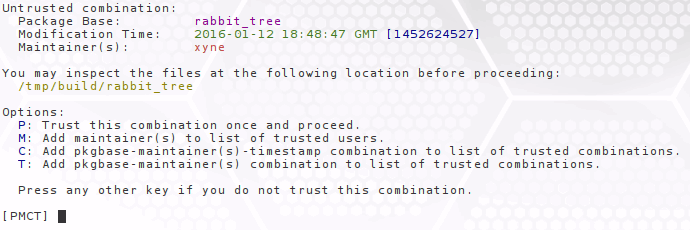
\includegraphics[width=\linewidth]{img/bb-query_trust-screenshot.png}
	\caption{Bauerbills trust management system \cite{bauerbill}}
	\label{fig:bb-query_trust}
\end{figure}

In the scenario from Section~\ref{sec:vcs_attack}, the assumption is that an upstreams VCS repository was attacked or made malicious changes.
No AUR helper is capable of detecting this attack because source integrity verification is normally handled my \texttt{makepkg}. If no checksums are available in the PKGBUILD, such as is the case for VCS packages, nothing can be done with the existing infrastructure.
However, \texttt{aursec} handles this exactly like it handles the previous attack because it hashes VCS sources in addition to the build files.

Therefore, \texttt{aursec} provides superior protection to existing solutions. The comparison is summarized in Table~\ref{tab:defence-comparison}.

\begin{table}
	\centering
	\begin{tabular}{l|m{3cm}|c|m{3cm}}
	\hline

	\hline
	\textbf{Detected Attack} & \textbf{AURsec} & \textbf{Bauerbill} & \textbf{aurutils} \\
	\hline
		Maintainer change & any change without new version & yes & no \\
		Modified build files & yes & manually & manually, diffs between versions \\
		Manipulated VCS sources & yes & no & no \\
	\hline

	\hline
	\end{tabular}
	\caption{Comparison of defence methods against our attack scenarios}
	\label{tab:defence-comparison}
\end{table}

% OTHER PACKAGE MANAGERS:
% EXPLAIN THAT THEY ARE INSECURE AS S**T
% AND THAT OUR APPROACH COULD BE ADAPTED TO THEM,
% allthough not as easily because the AUR has modular helpers already,
% whereas adapting to the other platforms would require forking/patching more monolithic tools or building custom ones

\subsection{Applicability to other packaging systems} % TODO: @lukas better wording instead of "community packaging systems"?
As noted in the introduction, other community packaging systems share security issues with the AUR, which means that most of the analysis from Section~\ref{sec:security_issues} also applies to them.
The \emph{Python Package Index} allows signing of packages with GPG, but its client (\texttt{pip}) cannot verify them~\cite{pypi:security}, so users would need to do that by hand.
There is also no web of trust or any similar mechanism, so users would need to build trust in every individual maintainer.
This is exactly the same situation as that of the AUR.

The \emph{Node package manager} is even worse: There is no means for any signing whatsoever~\cite{npm:security}.

Out of all community package managing systems we looked at, \emph{rubygems.org} is the only one that is open about the state of its security, but they also have the same problems:

\begin{displayquote}
RubyGems has had the ability to cryptographically sign gems since version 0.8.11. This signing works by using the gem cert command to create a key pair, and then packaging signing data inside the gem itself. The gem install command optionally lets you set a security policy, and you can verify the signing key for a gem before you install it.

However, this method of securing gems is not widely used. It requires a number of manual steps on the part of the developer, and there is no well-established chain of trust for gem signing keys. Discussion of new signing models such as X509 and OpenPGP is going on in the rubygems-trust wiki, the RubyGems-Developers list and in IRC.~\cite{rubygems:security}
\end{displayquote}

The communities of the above community packaging systems have been talking about security improvements for years (since about 2012 in most cases), but no significant work has been done to this day.
Since it works purely on the client side and doesn't require any modifications to infrastructure, the solution implemented by AURsec would also be applicable to these other systems.

However, it would take much more work than for the AUR because of the different nature of the ecosystems.
While the AUR is one central location, there is no official client for it, so many users use it by hand and a wide range of (often easily extensible) AUR helpers is available.
This makes it comparatively easy for people to use \texttt{aursec} with their existing workflow.
In contrast, the other community packaging systems each have \emph{one} monolithic official client, and none of them have sufficient hook or plugin mechanisms to make them extensible enough for something like AURsec, so adapting our work to those platforms would require creating custom clients or the distribution of patched versions of the official ones.


  \section{Discussion}
    \label{sec:discuss}
Simulated attacks of the kind discussed in Section \ref{sec:attack_scenarios} have been detected effectively in our experiments, and the core toolchain is convenient to use and performant.
Also synchronization between users and automatic mining works as expected.

However, our approach has several major disadvantages that necessarily follow from using a blockchain: Every user must have a full copy of the chain on his machine, which requires a non-negligible amount of hard drive memory at best.
The local copies must also be kept in sync, which requires a background process and near-permanent network connection.
Finally, the fact that we need a high mining difficulty to prevent the spreading of fake hashes makes our system very computationally expensive for what it is.

\subsection{Alternatives}
There are other conceivable ways of securing the AUR on the user side.
The most obvious one would be to do away with the blockchain and replace it with a traditional database accessible through a web service.

That approach has the advantage of being much lighter and more straightforward to use, as it doesn't need local blockchain copies, background processes or periodic mining on every client machine. However, it achieves that by creating a single point of failure (the web service) and a new trust requirement (in the owners of the web service).

In the end, the choice between these approaches involves a trade-off between computational costs and client-side complexity on the one hand, and basic trust on the other.

Other approaches would be the creation of a new, trusted source repository downstream of the AUR, requiring trust in a central authority, or a complete re-design of the AUR itself at the cost of ease of use. Neither of these is particularly appealing, allthough the former is very sensible for specific uses and/or closed organizations, and is already being used for those cases.


\subsection{Future Work}
The system would need several months of testing with hundreds of users in order to assess its actual performance, so we are looking forward to more engagement from the community when AURsec advances.
To date, we have not received enough feedback or run our project with enough people to draw meaningful conclusions.

However, we have already started working on a large update that will make the system more secure.
The main improvement is an extended smart contract that does not merely return the most common hash and its submission count, but also returns the count for the second most common hash.

This will allow us to factor the proportion between the two counts into the trust instead of the current simple trust threshold.
We also need to address the mining difficulty: that is, the system must be usable, but at the same time hard to manipulate. This will require more testing.
Depending on the mining difficulty that we choose, we might also make the periodic mining mine for a set time instead of a set number of blocks, in order to adjust the mining-effort of each user .
Finally, we want to use Systemd's cgroups resource management more effectively in order to limit the performance and battery impact of running our project in the background.


  % TODO: conclusion:

  \appendix
  \section{A sample \texttt{PKGBUILD}}\label{sec:our-pkgbuild}

\begin{minted}[linenos]{bash}
# Maintainer: Bennett Piater <bennett at piater dot name>

pkgname=(aursec-git aursec-tui-git)
pkgver=v0.11.r0.15ea0e9
pkgrel=1
pkgdesc='Verify AUR package sources against hashes stored in a blockchain.'
arch=(any)
url="https://github.com/clawoflight/${pkgbase%-git}"
license=('custom:MPL2')

provides=("${pkgname%-git}")
conflicts=("${pkgname%-git}")

depends=(firejail geth vim bc)
makedepends=(pandoc git)
checkdepends=(shellcheck)

source=("git+https://github.com/clawoflight/${pkgname%-git}.git")
sha256sums=('SKIP')
validpgpkeys=('871F10477DB3DDED5FC447B226C7E577EF967808')

pkgver() {
    cd "${pkgname%-git}"
    printf "%s" "$(git describe --long | sed 's/\([^-]*-\)g/r\1/;s/-/./g')"
}

build() {
    cd "${pkgname%-git}/aursec"
    make
    cd "../tui"
    make
}

check() {
    cd "${pkgname%-git}/aursec"
    make -k check
}

package_aursec-git() {
    install=aursec-git.install
    optdepends=("aursec-tui: to manually inspect the blockchain.")

    cd "${pkgname%-git}/aursec"
    make PREFIX="/usr" DESTDIR="$pkgdir/" install
}

package_aursec-tui-git() {
    pkgdesc='Inspect the aursec blockchain'
    depends=(python python-requests python-urwid aursec)
    provides=(aursec-tui)
    conflicts=(aursec-tui)

    cd "aursec/tui"
    make PREFIX="/usr" DESTDIR="$pkgdir/" install
}
\end{minted}

\section{Smart Contract}\label{sec:contract}
\begin{minted}[linenos]{javascript}
// This Source Code Form is subject to the terms of the Mozilla Public
// License, v. 2.0. If a copy of the MPL was not distributed with this
// file, You can obtain one at http://mozilla.org/MPL/2.0/.
// Copyright 2016-2017 Lukas Krismer and Bennett Piater.

pragma solidity ^0.4.0;
import "contracts/Owned.sol";

/**
 * @title Registry of AUR package hashes
 * @author Bennett Piater
 */
contract AURPackageRegistry is Owned {

    // Struct that holds the consensus
    // and the number of submissions for each hash for a package.
    struct PackageData {
        string currentConsensusPkgHash;
        mapping (string => uint) timesHashSubmitted;
    }

    // Map package IDs "$pkgname-$pkgver-$pkgrel" to the corresponding struct
    mapping (string => PackageData) packages;

    // Map a hash to a map of blockchain wallet addresses (users).
    // This allows checking whether a user submitted a hash.
    mapping (string => mapping (address => bool)) addressesThatSubmittedAHash;

    event PkgHashSubmitted(string indexed packageID, string pkgHash,
        uint submissionCount, address indexed submitter);
    event ConsensusFormed(string indexed packageID, string pkgHash,
        uint submissionCount);

    /**
     * @notice Get the current consensus and how many nodes submitted it
     * for a given package,version,release combination.
     *
     * @param packageID The id of the package to submit: pkgname-pkgver-pkgrel
     *
     * @return pkgHash The hash of the package, or the empty string if none is stored.
     * @return submissionCount The number of nodes that submitted this hash
     */
    function getCurrentConsensus(string packageID) constant
    returns (string pkgHash, uint submissionCount) {
        string hash = packages[packageID].currentConsensusPkgHash;
        return (hash, packages[packageID].timesHashSubmitted[hash]);
    }

    /**
     * @notice Submit a new hash for a package.
     *
     * @param packageID The id of the package to submit: pkgname-pkgver-pkgrel
     * @param pkgHash The hash of the package
     * @return success Whether the submission succeeded
     */
    function submitPkgHash(string packageID, string pkgHash) returns (bool success) {
        // Only allow every address (=user) to submit a hash once
        if (addressesThatSubmittedAHash[pkgHash][msg.sender])
            return false;
        addressesThatSubmittedAHash[pkgHash][msg.sender] = true;

        PackageData package = packages[packageID];
        package.timesHashSubmitted[pkgHash] += 1;
        // Trigger notification
        PkgHashSubmitted(packageID, pkgHash,
            package.timesHashSubmitted[pkgHash], msg.sender);

        // If this hash has become the new consensus
        if (package.timesHashSubmitted[pkgHash] >
            package.timesHashSubmitted[package.currentConsensusPkgHash]) {

            package.currentConsensusPkgHash = pkgHash;
            // Trigger notification
            ConsensusFormed(packageID, pkgHash, package.timesHashSubmitted[pkgHash]);
        }

        return true;
    }
}
\end{minted}

\newpage
\section{Adding Bootnodes}\label{sec:init-boot}
This section explains how mining and non-mining bootnodes can be created and integrated into our network.\newline

\textbf{Mining bootnodes} can only be initialized automatically with \emph{aursec-init} on Arch Linux.
After doing so, instead of starting the systemd services, use the command
\begin{verbatim}
sudo su aursec -c '/usr/bin/geth --fast --port 30200 --rpcport 8105 --nodiscover
--ipcdisable --rpc --rpcapi "eth,web3,miner" --datadir /var/aursec/chain --cache 512
--networkid 42 --verbosity 4 --unlock 0 --password /var/aursec/password console'
\end{verbatim}

to get a geth console. To get your node-url run \texttt{admin.nodeInfo}. Copy the url and close the console (Ctrl+D or exit). To start the node use

\begin{verbatim}
sudo su aursec -c '/usr/bin/geth --fast --port 30200 --rpcport 8105 --nodiscover
--ipcdisable --rpc --rpcapi "eth,web3,miner" --datadir /var/aursec/chain --cache 512
--networkid 42 --verbosity 4 --unlock 0 --password /var/aursec/password'
\end{verbatim}

Now start the \texttt{aursec-blockchain-mine.timer}.
To integrate the bootnode to the network, read the corresponding paragraph below.\linebreak

\textbf{Non-mining bootnodes} only require the \texttt{geth} package and can be set up on any system.
To initialize the bootnode run the following commands:
\begin{verbatim}
> bootnode -genkey $PathToKeyfile
> bootnode -nodekey $PathToKeyfile -addr 30200
\end{verbatim}
The node-url will be shown in the first line after the second command.
To integrate the bootnode into the network, read the following paragraph.


\paragraph*{Integrate the Bootnode}
Copy the node-url consisting of \texttt{nodeUrl@yourip:30200} to our \texttt{aursec-blockchain.service} \footnote{https://github.com/clawoflight/aursec/blob/master/aursec/lib/aursec-blockchain.service} after the \texttt{--bootnodes} argument and submit a pull request.


\newpage
\section{Contributions}\label{sec:resp}
We split our work into areas of responsibility for which one of us was responsible (see Table \ref{tab:responsibilities}). However, usually both of us worked on any given area.
\begin{table}[!htb]
\centering
\caption{Contributions}
\label{tab:responsibilities}
\begin{tabular}{|l|L{5.5cm}|L{5.5cm}|}
\hline
Name & Code &  Paper \\ \hline
Bennett Piater & Solidity (Smart Contracts), automatic mining, hashing of packages, main command pipeline , aurutils wrapper, AUR-Packages   &
Abstract,
Motivation (Complete Section \ref{sec:motivation}),
AURsec (Main tool up to and including architecture, Systemd services, Integration with AUR Helpers ) ( \Cref{sec:aursec,sec:aur-architecture,sec:aursec-systemd,sec:integration} including Appendix \ref{sec:our-pkgbuild}),
Solidity code (Appendix \ref{sec:contract}),
Evaluation (Complete Section \ref{sec:eval}),
Discussion (Complete Section \ref{sec:discuss})
\\ \hline
Lukas Krismer &  Initialization of the blockchain, Integration of the contract, bash-API for ethereum , Terminal-User-Interface, Initialization of the bootnode &
Forword,
Introduction (Complete Section \ref{sec:intro}),
Related Work (Complete Section \ref{sec:related}),
AURsec(workflow, blockchain implementation, initialization, API, Terminal User Interface, bootnode) ( \Cref{sec:AURsec,sec:workflow,sec:aur-block,sec:aursec-init,sec:aursec-chain,sec:tui} including Appendix \ref{sec:init-boot}),
Contributions (Appendix \ref{sec:resp})\\ \hline
\end{tabular}
\end{table}




  %%% Content ends here
  \pagebreak
  \bibliographystyle{plain}
  \bibliography{Literature.bib}

\end{document}
